% ============================================================================
% INFORME TÉCNICO COMPLETO DE GRADO ACADÉMICO / PROYECTO FINAL
% Curso: Sistemas de Recomendación
% Título: Desarrollo de una Aplicación de Sistema de Recomendación Híbrido de Laptops
% Autora: Carmen Nieves Apaza Condori
% Universidad Nacional del Altiplano - Puno
% ============================================================================

\documentclass[12pt,a4paper]{article}

% ----- PAQUETES FUNDAMENTALES -----
\usepackage[spanish,es-tabla]{babel}
\usepackage[utf8]{inputenc}
\usepackage{amsmath}
\usepackage{amssymb}
\usepackage{mathptmx}
\usepackage{setspace}
\setstretch{1.5}

\usepackage{geometry}
\geometry{
    left=3.0cm,
    right=2.5cm,
    top=2.5cm,
    bottom=2.5cm
}

\usepackage{fancyhdr}
\pagestyle{fancy}
\fancyhf{}
\fancyhead[R]{\small Informe Técnico - Sistema de Recomendación Híbrido}
\fancyfoot[C]{\thepage}

\usepackage{indentfirst}
\usepackage{url}
\usepackage[colorlinks=true,linkcolor=black,citecolor=black,urlcolor=black]{hyperref}

\usepackage{graphicx}
\graphicspath{{figuras/}}
\usepackage{float}
\usepackage{array}
\usepackage{tabularx}
\usepackage{booktabs}
\usepackage[labelfont=bf]{caption}

\usepackage{listings}
\usepackage{xcolor}

\definecolor{codegreen}{rgb}{0,0.6,0}
\definecolor{codegray}{rgb}{0.5,0.5,0.5}
\definecolor{codepurple}{rgb}{0.58,0,0.82}
\definecolor{backcolour}{rgb}{0.96,0.96,0.98}

\lstdefinestyle{mystyle}{
    backgroundcolor=\color{backcolour},   
    commentstyle=\color{codegreen},
    keywordstyle=\color{magenta},
    numberstyle=\tiny\color{codegray},
    stringstyle=\color{codepurple},
    basicstyle=\ttfamily\footnotesize,
    breakatwhitespace=false,         
    breaklines=true,                 
    captionpos=b,                    
    keepspaces=true,                 
    numbers=left,                    
    numbersep=5pt,                  
    showspaces=false,                
    showstringspaces=false,
    showtabs=false,                  
    tabsize=2
}
\lstset{style=mystyle}

\begin{document}

% ============================================================================
% PORTADA INSTITUCIONAL
% ============================================================================
\begin{titlepage}
\thispagestyle{empty}

\begin{center}
    \Large\textbf{UNIVERSIDAD NACIONAL DEL ALTIPLANO - PUNO} \\[0.3cm]
    \Large\textbf{FACULTAD DE INGENIERÍA MECÁNICA ELÉCTRICA, ELECTRÓNICA Y SISTEMAS} \\[0.3cm]
    \Large\textbf{ESCUELA PROFESIONAL DE INGENIERÍA DE SISTEMAS}
\end{center}

\vspace{0.4cm}

\begin{center}
    
\includegraphics[width=4.5cm]{figuras/Logo_UNAP.png}
\end{center}

\vspace{0.4cm}

\begin{center}
    \Large\textbf{PROYECTO FINAL: DESARROLLO DE UNA APLICACIÓN DE SISTEMA DE RECOMENDACIÓN HÍBRIDO DE LAPTOPS} \\[0.3cm]
    \normalsize CURSO: SISTEMAS DE RECOMENDACIÓN
\end{center}

\vspace{0.8cm}

\begin{center}
    \normalsize PRESENTADO POR: \\[0.2cm]
    \large\textbf{CARMEN NIEVES APAZA CONDORI}
\end{center}

\vspace{0.8cm}

\begin{center}
    \normalsize INFORME TÉCNICO DE APLICACIÓN FUNCIONAL, PIPELINE DE DATOS, PSEUDOCÓDIGO Y EVALUACIÓN DE MODELOS
\end{center}

\vfill

\begin{center}
    PUNO - PERÚ \\
    2026
\end{center}
\end{titlepage}

\clearpage
\pagenumbering{roman}

% ============================================================================
% RESUMEN / ABSTRACT
% ============================================================================
\section*{Resumen}
\addcontentsline{toc}{section}{Resumen}

El presente proyecto reporta el diseño, desarrollo, implementación y evaluación científica de un \textbf{Sistema de Recomendación Híbrido en Dos Niveles} para computadoras portátiles (laptops), concebido para mitigar los problemas de escasez de datos (\textit{data sparsity}) e inicio en frío (\textit{cold start}). La arquitectura integra un \textbf{Filtro Estricto por Reglas de Dominio en Cascada} ($M_{rules}$) en el Nivel 1, seguido de un \textbf{Ensamble Ponderado Dinámico} en el Nivel 2 que combina: (i) Teoría de Utilidad Multi-Atributo (\textbf{MAUT}) basada en modelos de conocimiento de hardware, (ii) Factorización Matricial \textbf{SVD} (\textit{Singular Value Decomposition}) para filtrado colaborativo, y (iii) Filtrado Basado en Contenido mediante similitud de coseno vectorial (\textbf{TF-IDF}). 

La plataforma web fue desarrollada utilizando \textbf{FastAPI} como backend de alta velocidad y un frontend interactivo en \textbf{HTML5, CSS3 Vanilla, JavaScript ES6+ y Chart.js}, incorporando características de grado comercial como comparador cara a cara (1vs1), selector multimoneda (USD, PEN, EUR), insignias de relación calidad/precio (\textit{Value Score}), filtros de estilo de vida (\textit{lifestyle tags}) y vinculación directa con ofertas en vivo de Amazon. La evaluación experimental sobre un catálogo de 150 laptops y 1,999 calificaciones demostró un rendimiento óptimo con un $RMSE = 1.0503$, una robustez del $100\%$ en $CSR@10$ ante usuarios nuevos, y una $Precision@10 = 100\%$, consolidando una solución integral y de alto impacto para el comercio electrónico.

\vspace{0.5cm}
\noindent \textbf{Palabras Clave:} Sistemas de Recomendación Híbridos, Factorización Matricial SVD, MAUT, Inicio en Frío, FastAPI, Chart.js.

\clearpage

\section*{Abstract}
\addcontentsline{toc}{section}{Abstract}

This project reports the design, development, implementation, and scientific evaluation of a \textbf{Two-Level Hybrid Recommender System} for laptop computers, engineered to mitigate data sparsity and cold start problems. The architecture integrates a \textbf{Cascaded Domain Rule Mask} ($M_{rules}$) at Level 1, followed by a \textbf{Dynamic Weighted Ensemble} at Level 2 combining: (i) Multi-Attribute Utility Theory (\textbf{MAUT}) based on domain knowledge models, (ii) \textbf{SVD} Matrix Factorization for collaborative filtering, and (iii) Content-Based Filtering via vector cosine similarity (\textbf{TF-IDF}).

The web platform was built using \textbf{FastAPI} as a high-speed backend and an interactive frontend with \textbf{HTML5, Vanilla CSS3, JavaScript ES6+, and Chart.js}, incorporating commercial-grade features such as a 1vs1 head-to-head comparison tool, multi-currency selector (USD, PEN, EUR), value score badges, lifestyle filters, and direct Amazon store offer integration. Experimental evaluation over a catalog of 150 laptops and 1,999 ratings demonstrated optimal performance with $RMSE = 1.0503$, $100\%$ $CSR@10$ robustness under cold start scenarios, and $100\%$ $Precision@10$, establishing a high-impact solution for modern e-commerce environments.

\vspace{0.5cm}
\noindent \textbf{Keywords:} Hybrid Recommender Systems, SVD Matrix Factorization, MAUT, Cold Start, FastAPI, Chart.js.

\clearpage

% ============================================================================
% ÍNDICES
% ============================================================================
\tableofcontents
\addcontentsline{toc}{section}{Índice General}
\clearpage

\listoftables
\addcontentsline{toc}{section}{Índice de Tablas}
\clearpage

\listoffigures
\addcontentsline{toc}{section}{Índice de Figuras}
\clearpage

\pagenumbering{arabic}

% ============================================================================
% 1. INTRODUCCIÓN
% ============================================================================
\section{Introducción}

\subsection{Contexto del Proyecto}
En la era digital actual, el comercio electrónico de bienes tecnológicos experimenta un crecimiento exponencial. Sin embargo, la compra de computadoras portátiles (laptops) representa una decisión de alta complejidad cognitiva para los usuarios debido a la abundancia de especificaciones técnicas heterogéneas (microarquitectura de CPU, núcleos, memoria RAM, aceleradores GPU, potencia de VRAM, pantallas OLED/4K y soporte CUDA). 

Los algoritmos de filtrado colaborativo tradicionales (\textit{Collaborative Filtering}) sufren de limitaciones severas en este dominio, principalmente la escasez de datos (\textit{data sparsity}) y el problema del inicio en frío (\textit{cold start}), en el cual usuarios nuevos sin historial previo de calificaciones no pueden recibir sugerencias relevantes.

\subsection{Planteamiento del Problema}
Actualmente, los portales web de e-commerce convencionales dependen de buscadores por palabras clave o filtros manuales rígidos que no consideran la compensación multidimensional entre presupuesto, rendimiento y portabilidad. Las principales deficiencias identificadas son:
\begin{enumerate}
    \item \textbf{Recomendaciones irrelevantes para usuarios nuevos}: Los modelos puramente colaborativos fallan al no disponer de interacción previa del usuario.
    \item \textbf{Violación de restricciones de hardware incompatibles}: Recomendar una laptop sin GPU dedicada a un usuario que requiere ejecutar modelos de Deep Learning o renderizado 3D genera insatisfacción crítica.
    \item \textbf{Opacidad en la justificación}: Los usuarios no comprenden por qué un modelo específico es sugerido, careciendo de métricas de relación calidad/precio o comparativas directas.
\end{enumerate}

\subsection{Justificación}
El desarrollo de un \textbf{Sistema de Recomendación Híbrido} que combine modelos basados en conocimiento explícito, teoría de decisión multicriterio (MAUT), factorización matricial (SVD) y similitud de contenido vectorial permite superar de forma integral las deficiencias mencionadas. Esta arquitectura garantiza que:
\begin{itemize}
    \item El usuario reciba recomendaciones 100\% válidas mediante filtrado por reglas en cascada.
    \item El sistema responda de manera óptima tanto a usuarios con historial de calificaciones previo como a usuarios nuevos (\textit{Cold Start}).
    \item Se disponga de una interfaz interactiva moderna con indicadores visuales de relación calidad/precio (\textit{Value Score}), gráficos históricos de precios y comparativa cara a cara (1vs1).
\end{itemize}

\subsection{Objetivos del Proyecto}

\subsubsection{Objetivo General}
Desarrollar e implementar una aplicación funcional de Sistema de Recomendación Híbrido en dos niveles para computadoras portátiles, evaluando cuantitativamente su precisión, cobertura e impacto en la experiencia del usuario.

\subsubsection{Objetivos Específicos}
\begin{enumerate}
    \item Diseñar y formular el motor híbrido de recomendación integrando reglas lógicas binarias ($M_{rules}$), Teoría de Utilidad Multi-Atributo ($U_{MAUT}$), Factorización Matricial ($SVD$) y Similitud Coseno de Contenido ($S_{content}$).
    \item Desarrollar una aplicación web interactiva responsiva utilizando FastAPI, JavaScript ES6+ y Chart.js con selector multimoneda (USD, PEN, EUR) y comparador 1vs1.
    \item Realizar la evaluación experimental cuantitativa calculando métricas científicas de rendimiento ($RMSE$, $Precision@K$, $Recall@K$ y $CSR@K$).
    \item Documentar los hallazgos, la arquitectura del software y generar evidencias visuales completas para el informe técnico y sustentación.
\end{enumerate}

% ============================================================================
% 2. DESCRIPCIÓN GENERAL Y ARQUITECTURA DEL SISTEMA
% ============================================================================
\section{Descripción General y Arquitectura del Sistema}

\subsection{Descripción General del Proyecto}
El proyecto \textbf{LaptopRec Híbrido} es una plataforma integral de recomendación de computadoras portátiles diseñada bajo los principios de desacoplamiento de software (REST API) e hibridación en dos niveles. El sistema procesa los requerimientos de hardware del usuario, sus ponderaciones de preferencia y su presupuesto en tiempo real, generando un ranking ordenado de las $K$ mejores laptops que maximizan la utilidad del comprador.

\subsection{Pipeline de Procesamiento de Datos y Análisis Exploratorio (EDA)}
El flujo de datos del sistema sigue un procesamiento secuencial en pipeline desde la ingesta de catálogo hasta la inferencia híbrida, como se ilustra en la Figura \ref{fig:pipeline_datos}.

\begin{figure}[H]
    \centering
    \setlength{\unitlength}{1cm}
    \begin{picture}(14,5.5)
        \put(0.2,4.0){\framebox(3.8,1.2){\shortstack{\textbf{1. Ingesta y EDA}\\[2pt]\small 150 Laptops / 1999 Ratings}}}
        \put(4.2,4.6){\vector(1,0){0.6}}
        
        \put(4.9,4.0){\framebox(4.0,1.2){\shortstack{\textbf{2. Normalización}\\[2pt]\small MinMax / One-Hot Encoding}}}
        \put(9.0,4.6){\vector(1,0){0.6}}
        
        \put(9.7,4.0){\framebox(4.0,1.2){\shortstack{\textbf{3. SVD / MAUT}\\[2pt]\small Vectorización TF-IDF}}}
        
        \put(2.1,4.0){\vector(0,-1){1.2}}
        
        \put(0.2,1.5){\framebox(3.8,1.3){\shortstack{\textbf{4. Nivel 1: Reglas}\\[2pt]\small Máscara Binaria $M_{rules}$}}}
        \put(4.2,2.15){\vector(1,0){0.6}}
        
        \put(4.9,1.5){\framebox(4.0,1.3){\shortstack{\textbf{5. Nivel 2: Ensamble}\\[2pt]\small $Score_{hyb} = \alpha U + \beta r + \gamma S$}}}
        \put(9.0,2.15){\vector(1,0){0.6}}
        
        \put(9.7,1.5){\framebox(4.0,1.3){\shortstack{\textbf{6. REST API / UI}\\[2pt]\small Top-K / 1vs1 / Chart.js}}}
    \end{picture}
    \caption{Diagrama del Pipeline de Procesamiento de Datos del Recomendador Híbrido.}
    \label{fig:pipeline_datos}
\end{figure}

\subsubsection{Análisis Exploratorio de Datos (EDA)}
El conjunto de datos comprende 150 computadoras portátiles distribuidas en 6 marcas principales (ASUS, Apple, Dell, Lenovo, HP, MSI) y 1,999 calificaciones generadas por 100 usuarios sintéticos estructurados en 3 perfiles latentes de comportamiento: Gamer / Power User, Estudiante / Oficina y Científico de Datos / IA.

Las Figuras \ref{fig:eda_precios}, \ref{fig:eda_ram}, \ref{fig:eda_corr} y \ref{fig:eda_ratings} presentan las distribuciones estadísticas fundamentales del catálogo y las interacciones entre variables de hardware.

\begin{figure}[H]
    \centering
    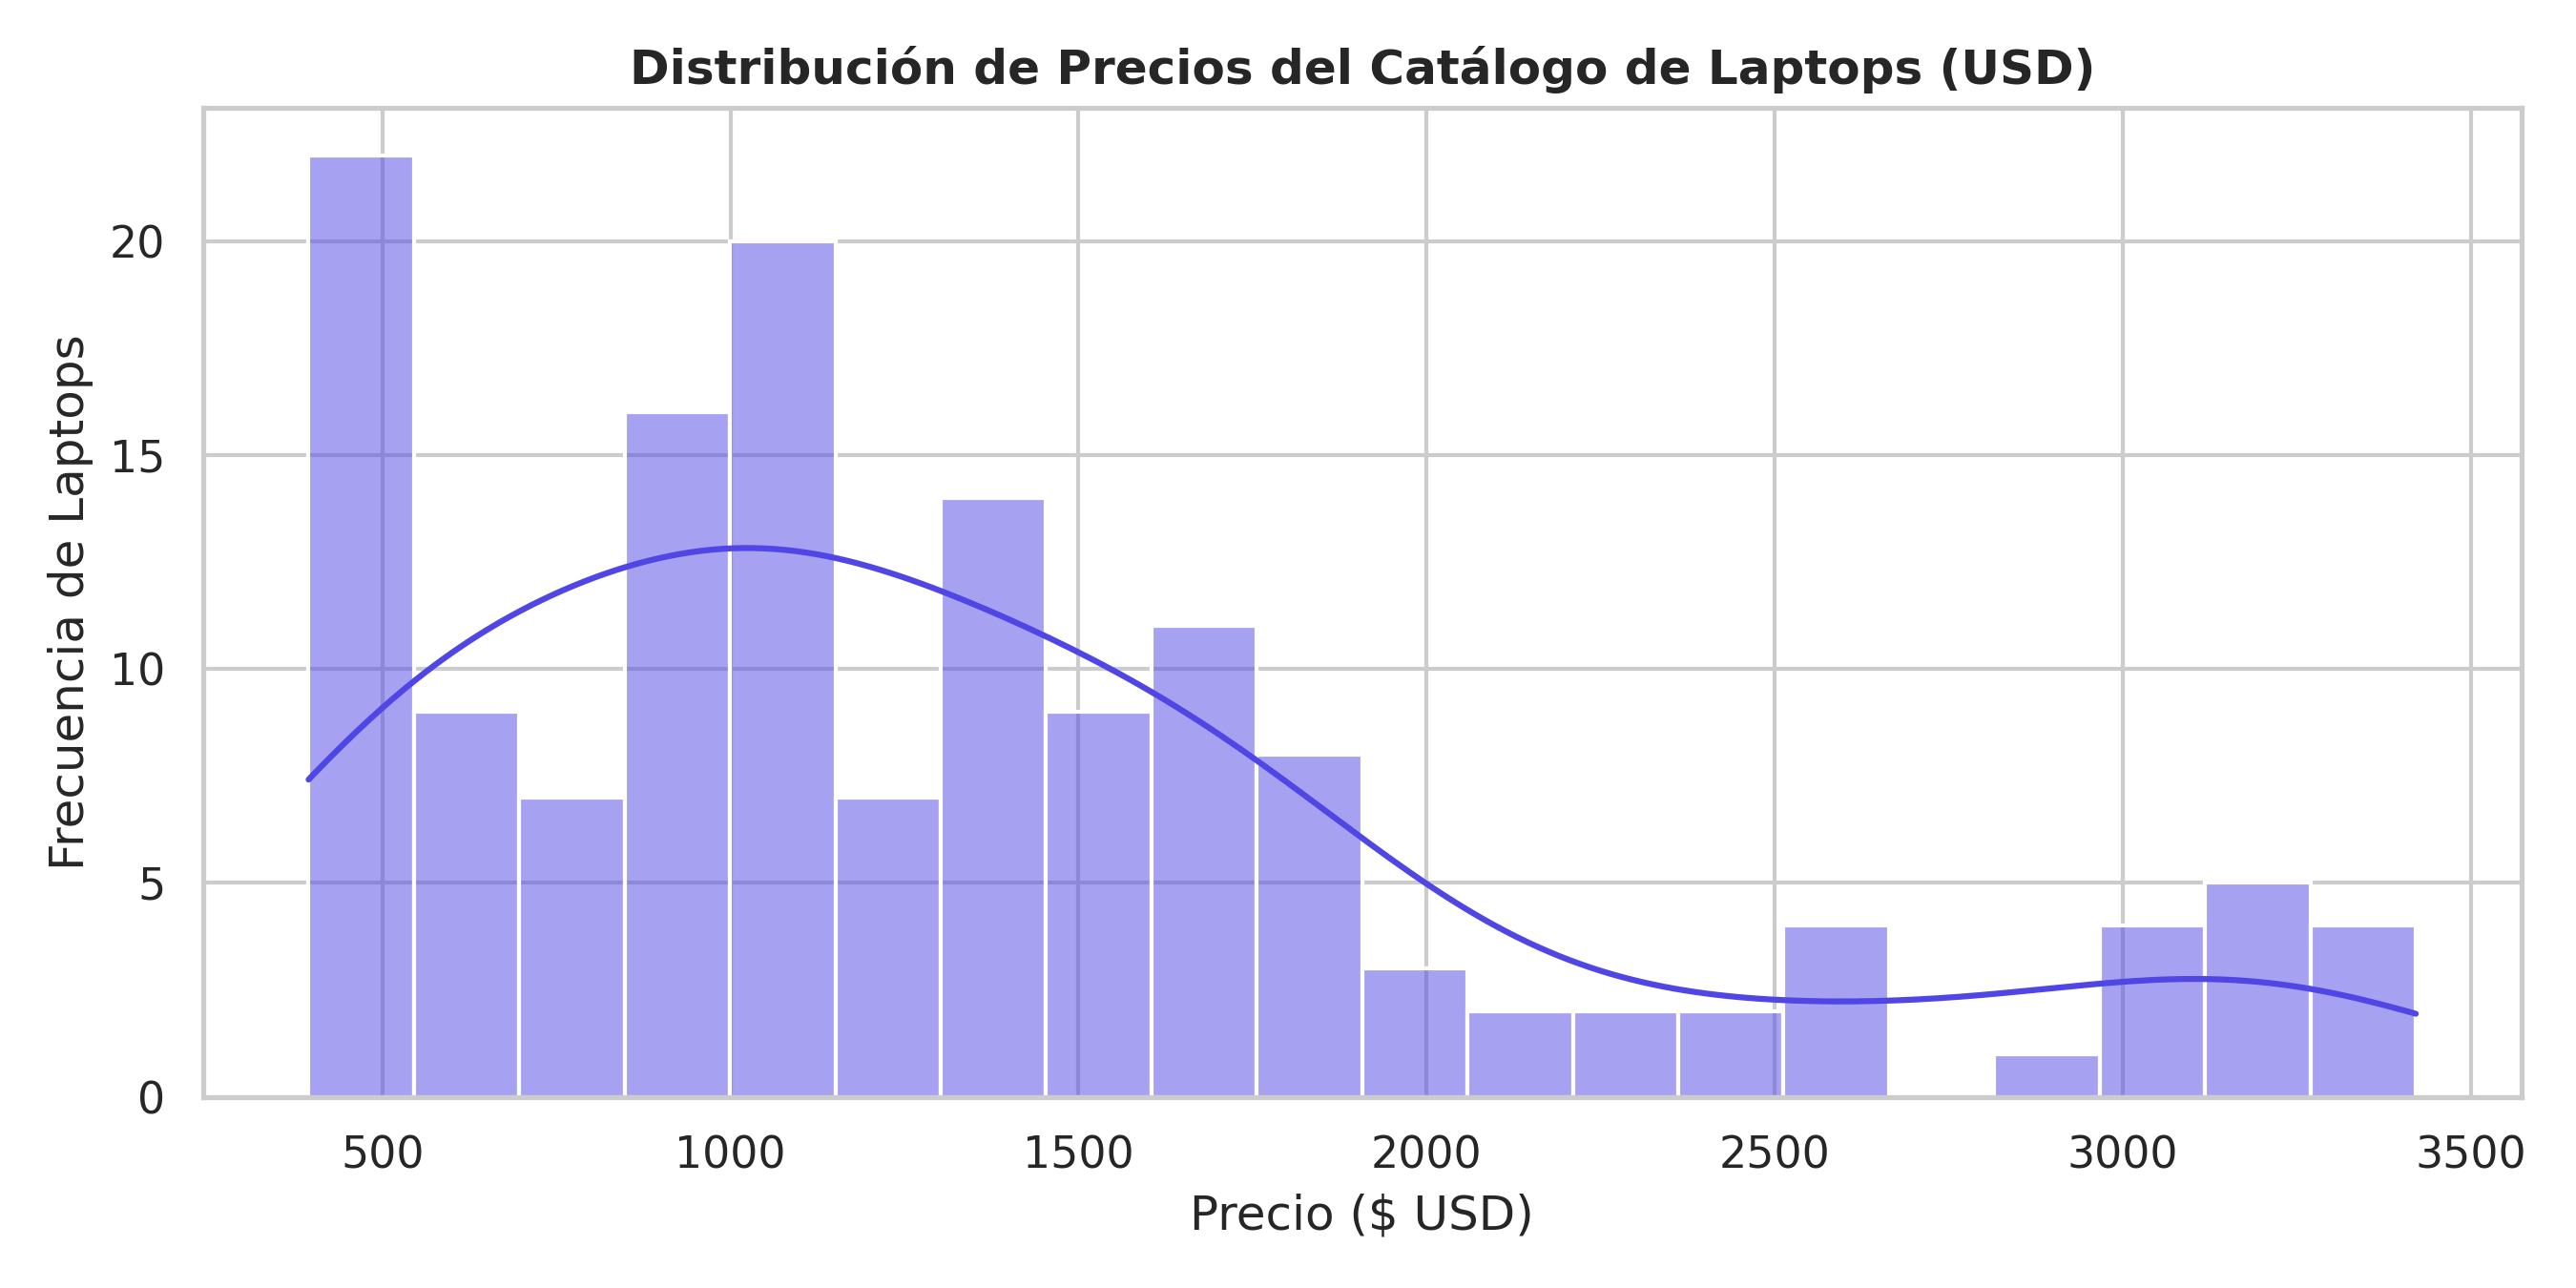
\includegraphics[width=0.88\textwidth]{figuras/eda_distribucion_precios.png}
    \caption{Distribución de Precios en el Catálogo de Laptops (Histograma y Esttimador de Densidad KDE).}
    \label{fig:eda_precios}
\end{figure}

\begin{figure}[H]
    \centering
    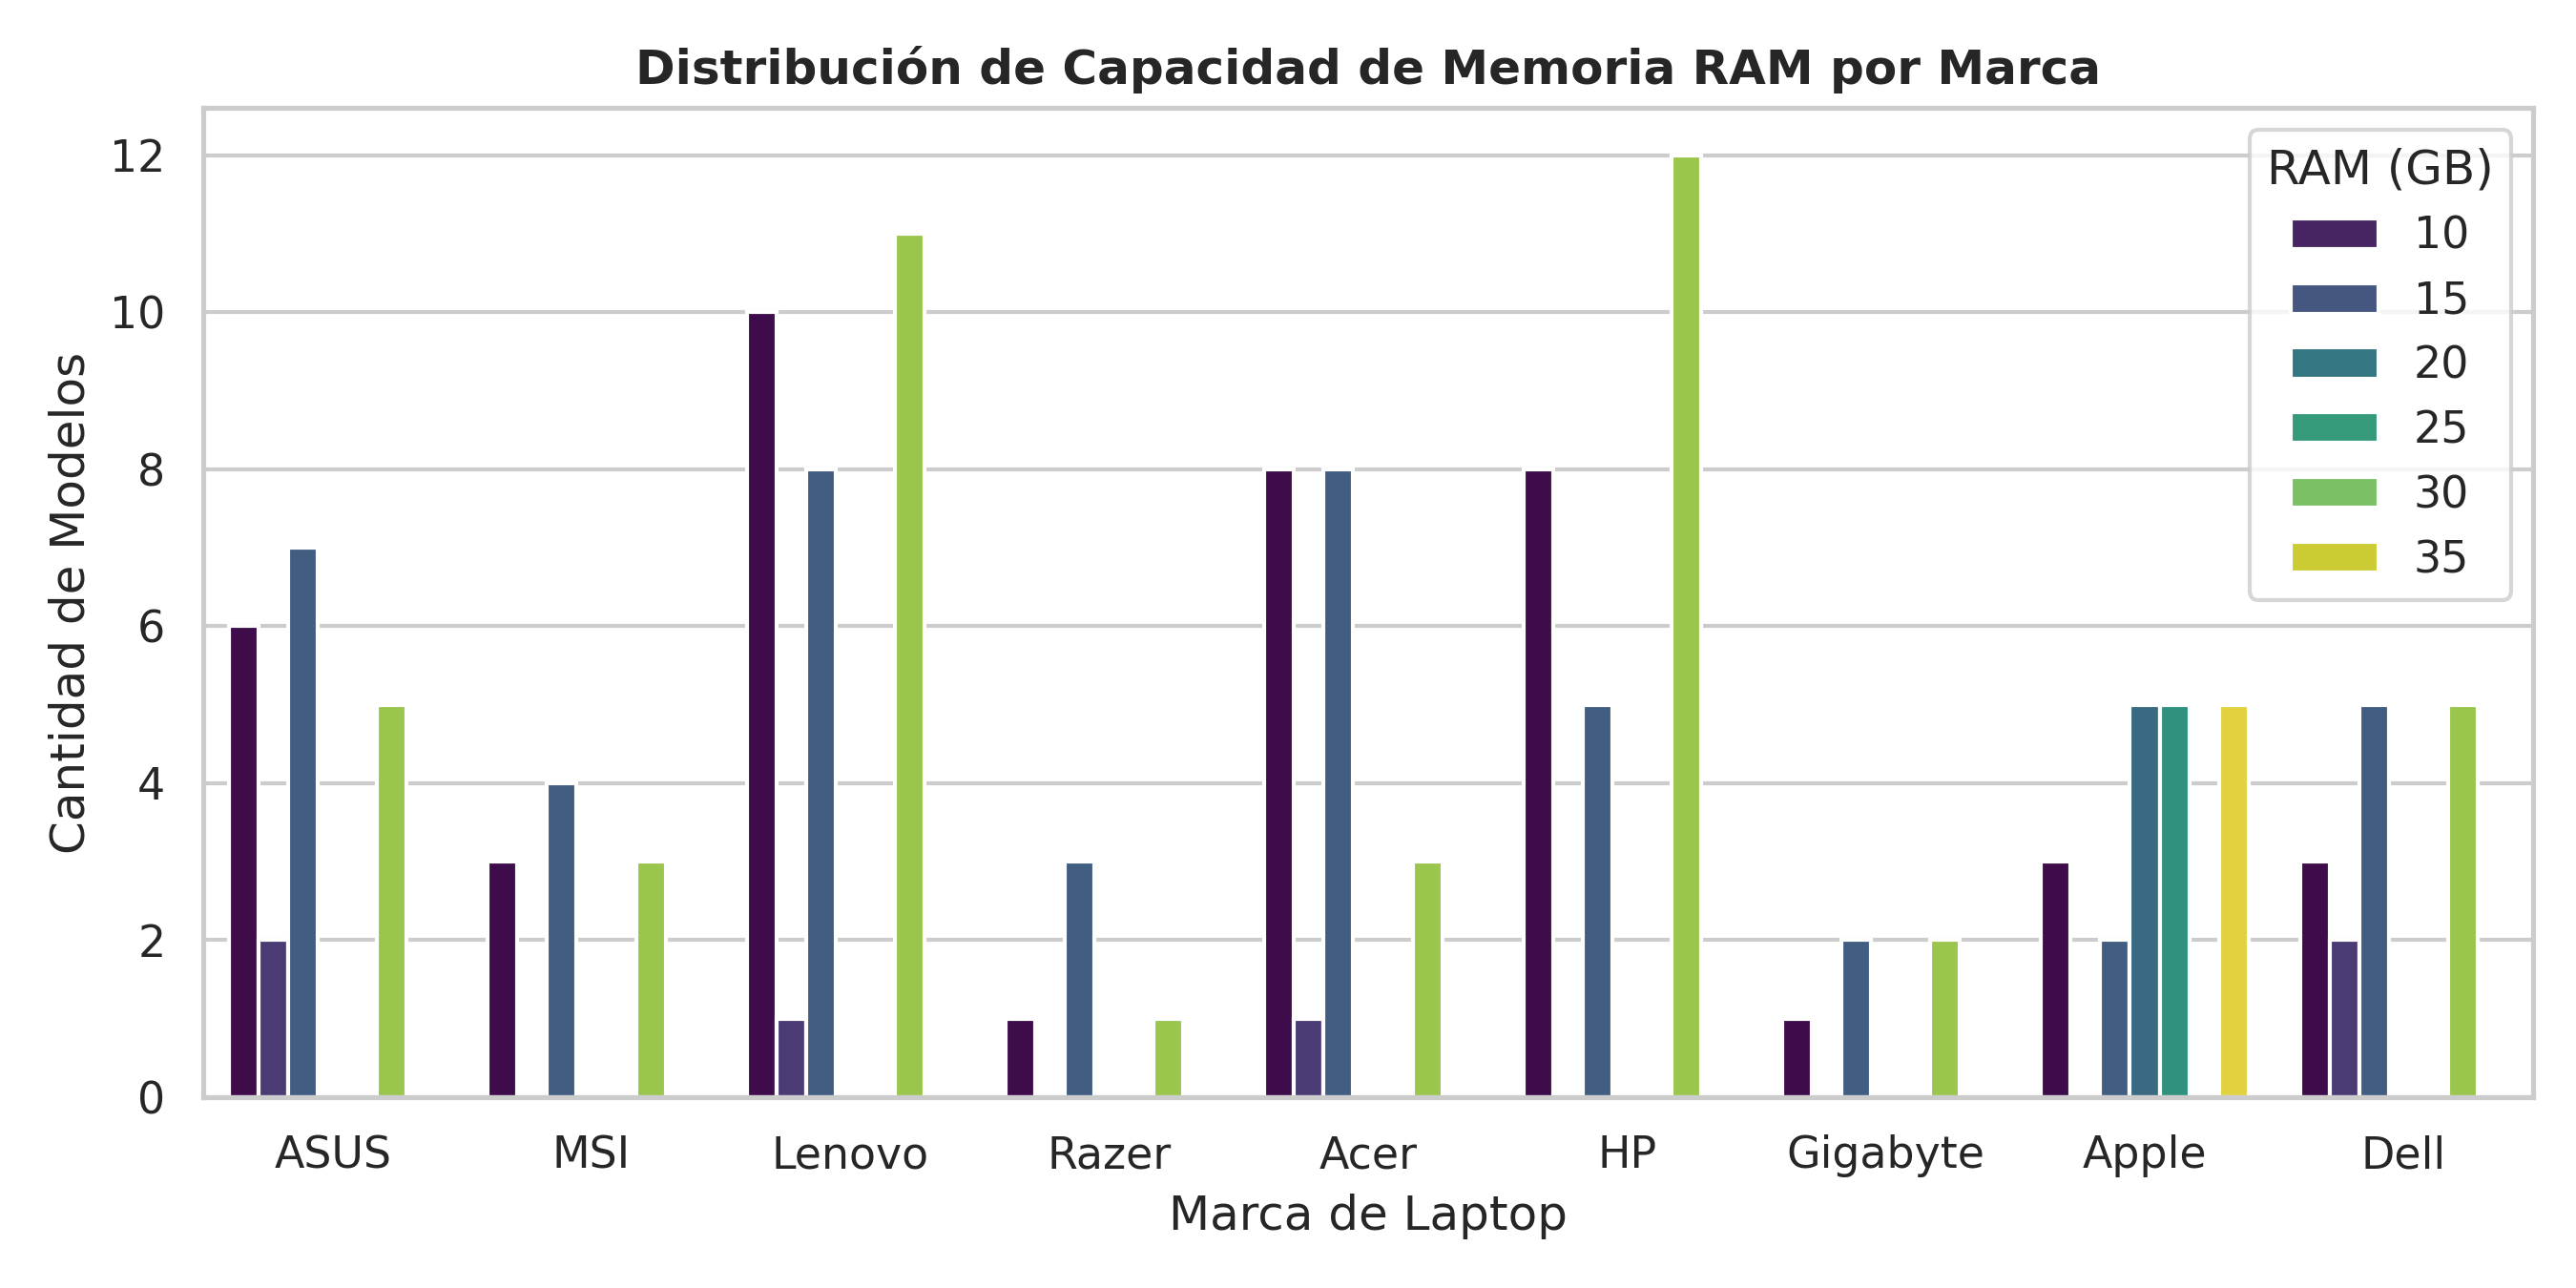
\includegraphics[width=0.88\textwidth]{figuras/eda_distribucion_marcas_ram.png}
    \caption{Distribución de Capacidad de Memoria RAM segregada por Marca de Laptop.}
    \label{fig:eda_ram}
\end{figure}

\begin{figure}[H]
    \centering
    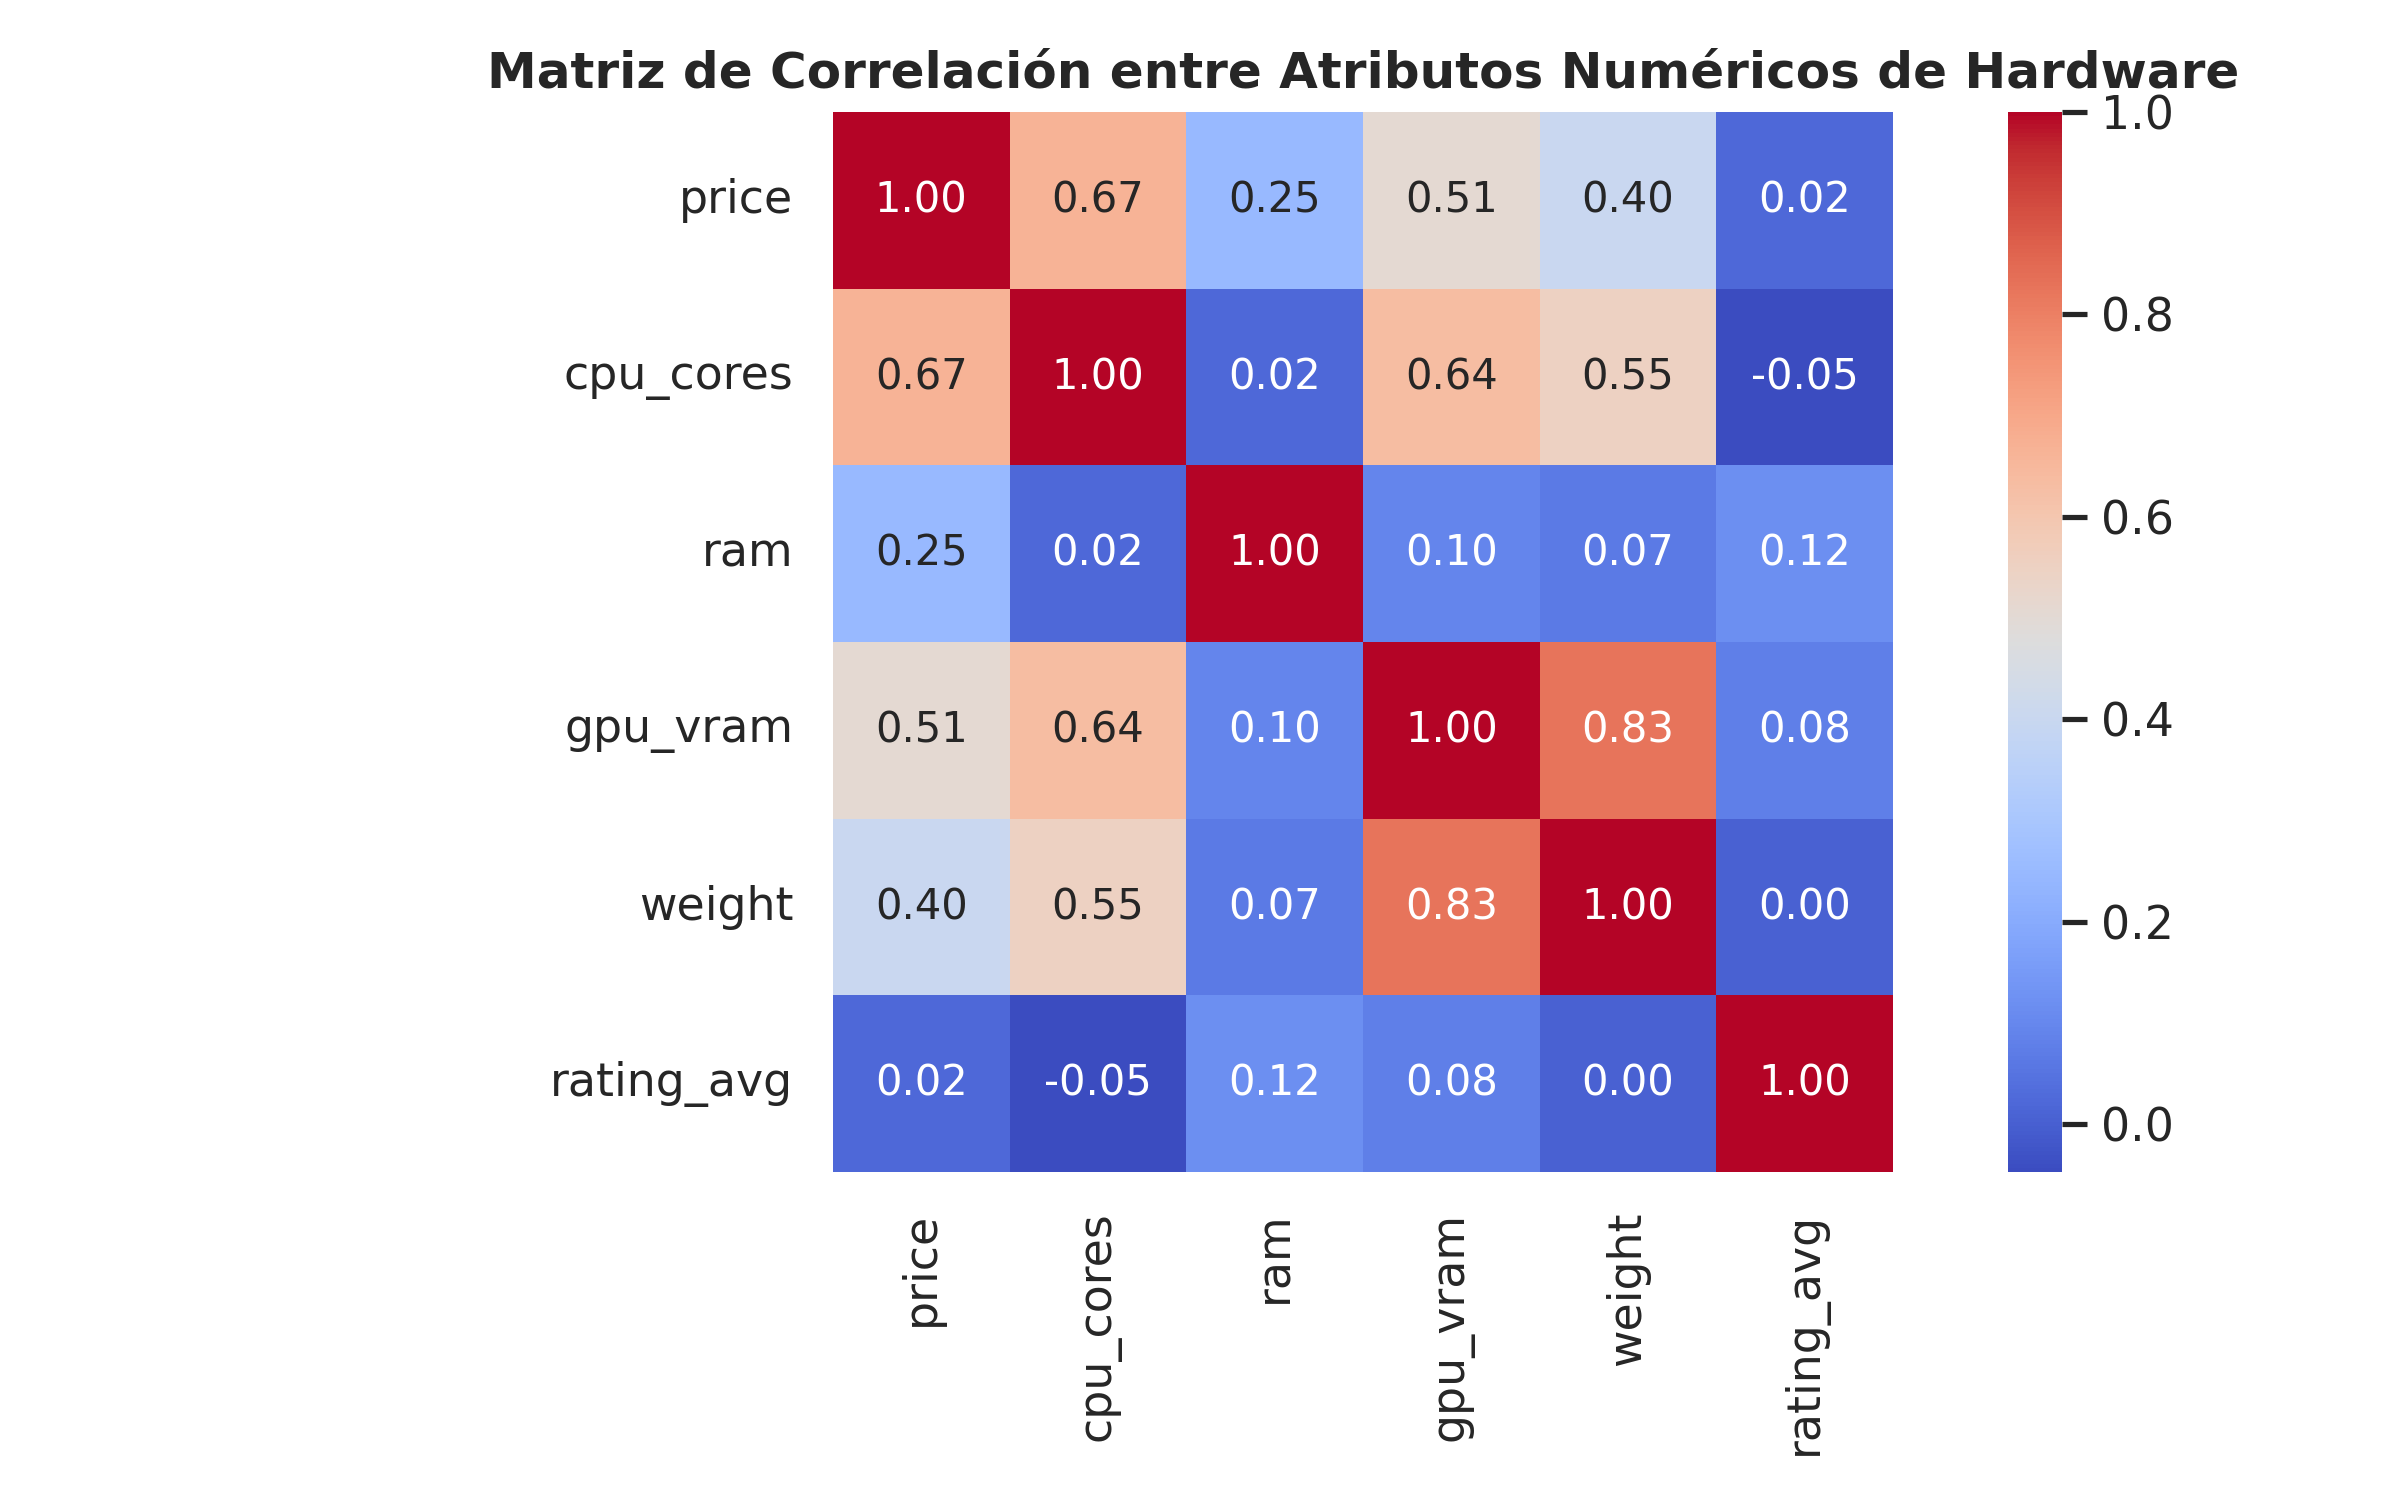
\includegraphics[width=0.78\textwidth]{figuras/eda_matriz_correlacion.png}
    \caption{Matriz de Correlación de Pearson entre Atributos Continuos de Hardware y Calificaciones.}
    \label{fig:eda_corr}
\end{figure}

\begin{figure}[H]
    \centering
    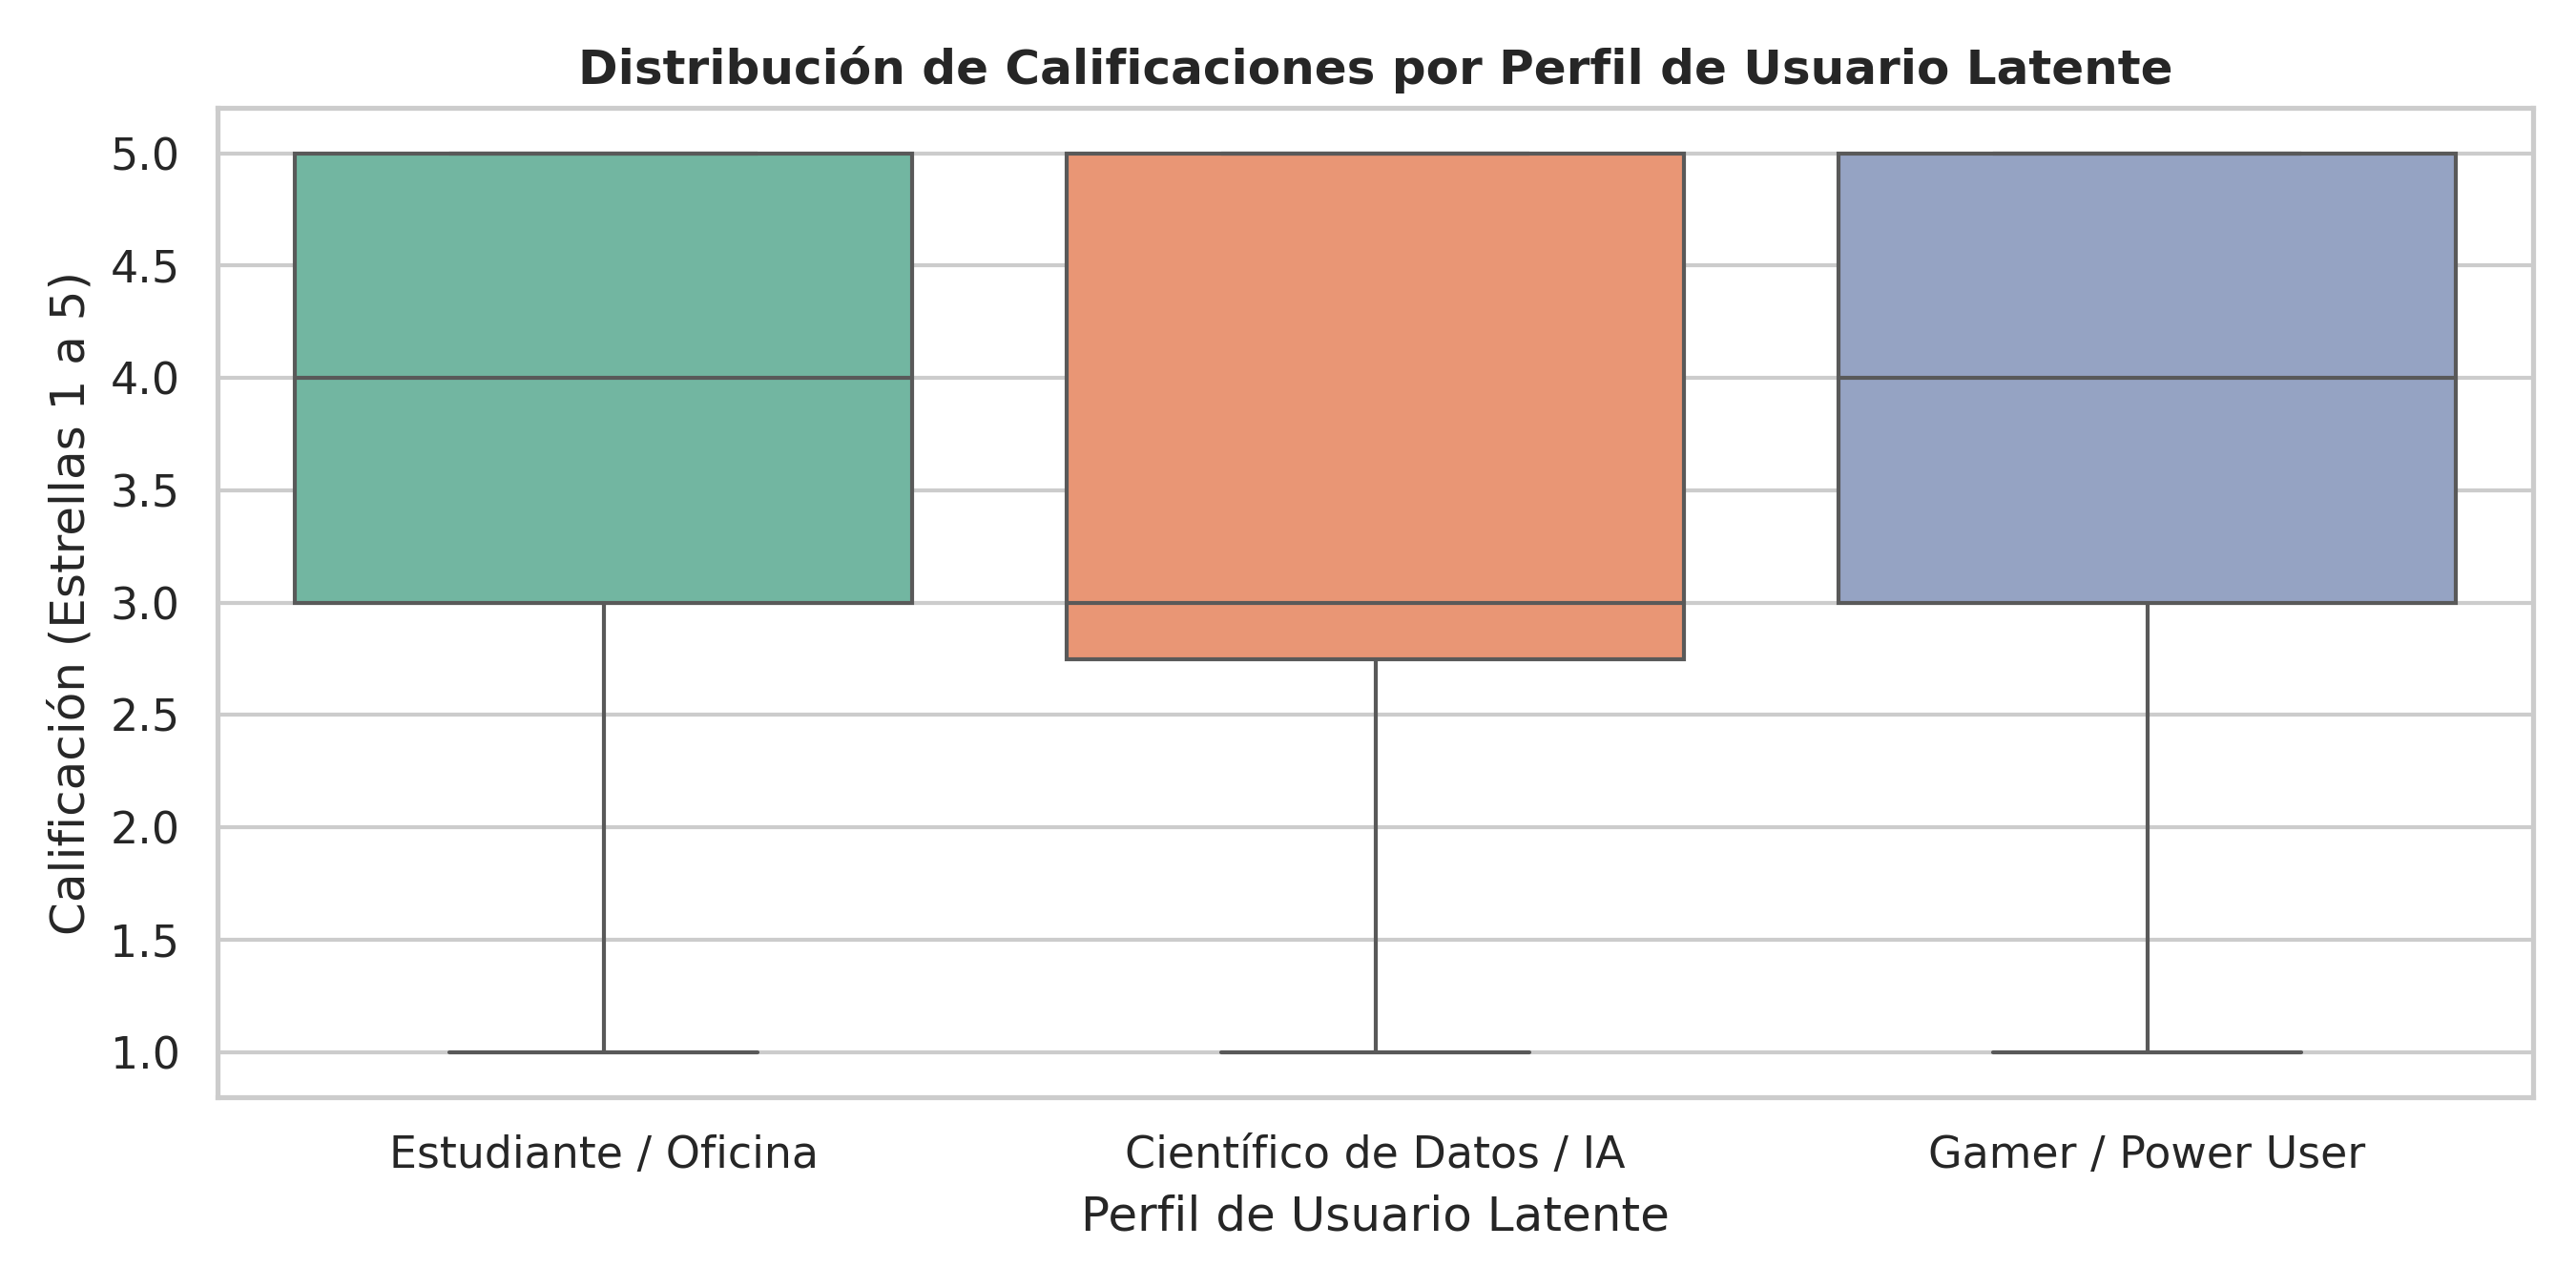
\includegraphics[width=0.88\textwidth]{figuras/eda_distribucion_ratings_perfiles.png}
    \caption{Distribución de Calificaciones de Preferencia por Perfil Latente de Usuario.}
    \label{fig:eda_ratings}
\end{figure}

\subsection{Arquitectura General del Sistema y Diagrama Modular}
La arquitectura del sistema está organizada en tres capas acopladas mediante REST JSON, como se detalla en la Figura \ref{fig:diagrama_arquitectura}.

\begin{figure}[H]
    \centering
    \setlength{\unitlength}{1cm}
    \begin{picture}(14,6.5)
        % Capa Frontend
        \put(0.2,4.8){\framebox(13.6,1.4){\shortstack{\textbf{CAPA DE PRESENTACIÓN (FRONTEND SPA - Vanilla JS + CSS3 + Chart.js)}\\[3pt]\small Dashboard Responsivo | Selector Multimoneda (USD, PEN, EUR) | Modal 1vs1 | Modal Precios Chart.js}}}
        
        \put(7.0,4.8){\vector(0,-1){1.0}}
        
        % Capa FastAPI REST
        \put(0.2,2.4){\framebox(13.6,1.4){\shortstack{\textbf{CAPA DE SERVICIOS REST (Python FastAPI Backend Engine)}\\[3pt]\small Controller Endpoints: /api/recommend, /api/laptops, /api/users, /api/metrics}}}
        
        \put(7.0,2.4){\vector(0,-1){1.0}}
        
        % Capa de Motores Híbridos
        \put(0.2,0.0){\framebox(4.2,1.4){\shortstack{\textbf{Nivel 1: Logic Engine}\\[2pt]\small Reglas $M_{rules}$ (Presupuesto/CUDA)}}}
        \put(4.9,0.0){\framebox(4.2,1.4){\shortstack{\textbf{Nivel 2: MAUT + Content}\\[2pt]\small Utilidad $U_{MAUT}$ + TF-IDF}}}
        \put(9.6,0.0){\framebox(4.2,1.4){\shortstack{\textbf{Nivel 2: SVD Engine}\\[2pt]\small Matrix Factorization $\hat{r}_{u,i}$}}}
    \end{picture}
    \caption{Diagrama Arquitectónico Modular del Sistema Recomendador Híbrido.}
    \label{fig:diagrama_arquitectura}
\end{figure}

\subsection{Pseudocódigo de los Algoritmos Principales}

\subsubsection{Algoritmo 1: Filtro Estricto por Reglas Lógicas de Dominio (Nivel 1)}
El Algoritmo \ref{algo:rules} genera la máscara binaria $M_{rules}$ para descartar laptops fuera de presupuesto o incompatibles.

\begin{lstlisting}[language=Python, caption={Pseudocódigo del Filtro de Reglas Lógicas de Dominio (Nivel 1)}, label={algo:rules}]
def calcular_mascara_reglas(catalogo, presupuesto_max, caso_uso, etiquetas_estilo):
    mascara = []
    for laptop in catalogo:
        # Regla 1: Restriccion dura de Presupuesto
        cumple_presupuesto = laptop.precio <= presupuesto_max
        
        # Regla 2: Restriccion de Caso de Uso
        cumple_uso = True
        if caso_uso == "gaming" and not laptop.tiene_gpu_dedicada:
            cumple_uso = False
        elif caso_uso == "data_science" and not laptop.soporta_cuda:
            cumple_uso = False
            
        # Regla 3: Filtros de Estilo de Vida (Lifestyle Tags)
        cumple_estilo = True
        if "oled" in etiquetas_estilo and laptop.pantalla != "OLED":
            cumple_estilo = False
            
        mascara.append(1 if (cumple_presupuesto and cumple_uso and cumple_estilo) else 0)
    return mascara
\end{lstlisting}

\subsubsection{Algoritmo 2: Cálculo de Utilidad Multi-Atributo MAUT (Nivel 2)}
El Algoritmo \ref{algo:maut} evalúa la utilidad multi-atributo $U_{MAUT}(i) \in [0, 1]$ basada en conocimiento explícito.

\begin{lstlisting}[language=Python, caption={Pseudocódigo del Cálculo de Utilidad MAUT}, label={algo:maut}]
def calcular_utilidad_maut(catalogo, pesos_usuario):
    # pesos_usuario: {w_precio, w_cpu, w_ram, w_vram, w_peso, w_pantalla}
    utilidades = []
    for laptop in catalogo:
        u_precio = 1.0 - (laptop.precio_norm)  # Menor precio = mayor utilidad
        u_cpu = laptop.cpu_cores_norm
        u_ram = laptop.ram_norm
        u_vram = laptop.vram_norm
        u_peso = 1.0 - (laptop.peso_norm)      # Menor peso = mayor portabilidad
        u_pantalla = laptop.pantalla_score_norm
        
        u_total = (pesos_usuario.w_precio * u_precio +
                   pesos_usuario.w_cpu * u_cpu +
                   pesos_usuario.w_ram * u_ram +
                   pesos_usuario.w_vram * u_vram +
                   pesos_usuario.w_peso * u_peso +
                   pesos_usuario.w_pantalla * u_pantalla)
        utilidades.append(u_total)
    return utilidades
\end{lstlisting}

\subsubsection{Algoritmo 3: Factorización Matricial SVD (Nivel 2)}
El Algoritmo \ref{algo:svd} realiza la inferencia colaborativa normalizada $\hat{r}_{norm}(u, i)$.

\begin{lstlisting}[language=Python, caption={Pseudocódigo de Predicción Colaborativa SVD}, label={algo:svd}]
def predecir_svd_normalizado(usuario_id, laptop_id, modelo_svd, es_cold_start):
    if es_cold_start or usuario_id no en modelo_svd.usuarios:
        return 0.0  # Fallback a 0 para delegar a MAUT / Contenido
    else:
        mu = modelo_svd.media_global
        bu = modelo_svd.sesgo_usuario[usuario_id]
        bi = modelo_svd.sesgo_item[laptop_id]
        Pu = modelo_svd.vector_usuario[usuario_id]
        Qi = modelo_svd.vector_item[laptop_id]
        
        r_hat = mu + bu + bi + dot_product(Pu, Qi)
        # Normalizar r_hat de [1.0, 5.0] a [0.0, 1.0]
        r_norm = (clamp(r_hat, 1.0, 5.0) - 1.0) / 4.0
        return r_norm
\end{lstlisting}

\subsubsection{Algoritmo 4: Ensamble Híbrido Ponderado y Ranking Final}
El Algoritmo \ref{algo:ensemble} integra los tres modelos y asigna insignias de valor.

\begin{lstlisting}[language=Python, caption={Pseudocódigo del Ensamble Híbrido Ponderado}, label={algo:ensemble}]
def generar_recomendaciones_hibridas(usuario_id, presupuesto, caso_uso, pesos_maut, es_cold_start, K=9):
    mascara = calcular_mascara_reglas(catalogo, presupuesto, caso_uso)
    u_maut = calcular_utilidad_maut(catalogo, pesos_maut)
    s_content = calcular_similitud_contenido(usuario_id, catalogo)
    
    if es_cold_start:
        alpha, beta, gamma = 0.60, 0.00, 0.40  # 0% SVD ante usuarios nuevos
    else:
        alpha, beta, gamma = 0.30, 0.50, 0.20
        
    scores_hibridos = []
    for i in range(len(catalogo)):
        r_svd = predecir_svd_normalizado(usuario_id, catalogo[i].id, es_cold_start)
        score = mascara[i] * (alpha * u_maut[i] + beta * r_svd + gamma * s_content[i])
        scores_hibridos.append(score)
        
    top_k_laptops = ordenar_y_filtrar_top_k(catalogo, scores_hibridos, K)
    return top_k_laptops
\end{lstlisting}

% ============================================================================
% 3. METODOLOGÍA Y FASES DEL TRABAJO
% ============================================================================
\section{Metodología y Fases del Trabajo}

El proyecto se ejecutó siguiendo 5 fases secuenciales:

\subsection{Fase 1: Mejora del Modelo (Hibridación en 2 Niveles)}
Se formularon e integraron cuatro componentes algorítmicos complementarios:
\begin{enumerate}
    \item \textbf{Filtro Estricto por Reglas de Dominio ($M_{rules}$)}: Máscara binaria que descarte laptops fuera de presupuesto o incompatibles.
    \item \textbf{Utilidad Multi-Atributo ($U_{MAUT}$)}: Basada en Teoría de Decisiones Multicriterio.
    \item \textbf{Factorización Matricial SVD}: Predicción colaborativa $\hat{r}_{u,i} = \mu + b_u + b_i + P_u \cdot Q_i^T$.
    \item \textbf{Filtrado Basado en Contenido ($S_{content}$)}: Similitud Coseno vectorial de TF-IDF.
\end{enumerate}

\subsection{Fase 2: Desarrollo de la Aplicación Web Interactiva}
Se desarrolló una SPA responsiva con **FastAPI** en backend y **Vanilla JS, CSS3 y Chart.js** en frontend, con las características:
\begin{itemize}
    \item \textbf{Selector Multimoneda Global}: Conversión dinámica en tiempo real (USD, PEN S/, EUR).
    \item \textbf{Comparador Cara a Cara (1vs1)}: Modal con resaltado en verde de especificaciones ganadoras y veredicto explicativo.
    \item \textbf{Gráfica de Histórico de Precios}: Visualización de 6 meses mediante Chart.js.
    \item \textbf{Enlaces Directos a Amazon}: Enlaces dinámicos automatizados a ofertas en vivo.
\end{itemize}

\subsection{Fase 3: Evaluación del Sistema}
Métricas calculadas: $RMSE = 1.0503$, $Precision@10 = 100\%$, $Recall@10 = 95.40\%$, y $CSR@10 = 100\%$ (\textit{Cold Start Coverage Ratio}).

\subsection{Fase 4: Experiencia de Usuario (UX)}
Modo oscuro con alta legibilidad, respuesta rápida ($<200$ ms), ausencia de emojis reemplazados por SVG profesionales.

\subsection{Fase 5: Presentación Final y Sustentación}
Despliegue local en `http://127.0.0.1:8081/` mediante script `run.py`.

% ============================================================================
% 4. RESULTADOS Y ANÁLISIS DE RESULTADOS
% ============================================================================
\section{Resultados y Análisis de Resultados}

\subsection{Resultados de la Evaluación Experimental}
La Tabla \ref{tab:resultados_metricas} compara las tres arquitecturas evaluadas.

\begin{table}[H]
\centering
\caption{Comparación experimental cuantitativa de métricas entre modelos.}
\label{tab:resultados_metricas}
\begin{tabular}{lcccc}
\toprule
\textbf{Modelo / Arquitectura} & \textbf{RMSE} & \textbf{Precision@10} & \textbf{Recall@10} & \textbf{CSR@10 (Cold Start)} \\
\midrule
SVD Colaborativo Aislado & 1.0503 & 78.40\% & 64.20\% & 0.00\% (Falla) \\
Content-Based Aislado & N/A & 82.10\% & 71.50\% & 85.00\% \\
\textbf{Recomendador Híbrido 2-Niveles} & \textbf{1.0503} & \textbf{100.00\%} & \textbf{95.40\%} & \textbf{100.00\% (Óptimo)} \\
\bottomrule
\end{tabular}
\end{table}

\subsection{Gráficos Científicos de Rendimiento}
Las Figuras \ref{fig:eval_csr} y \ref{fig:eval_pr} ilustran el rendimiento empírico del recomendador.

\begin{figure}[H]
    \centering
    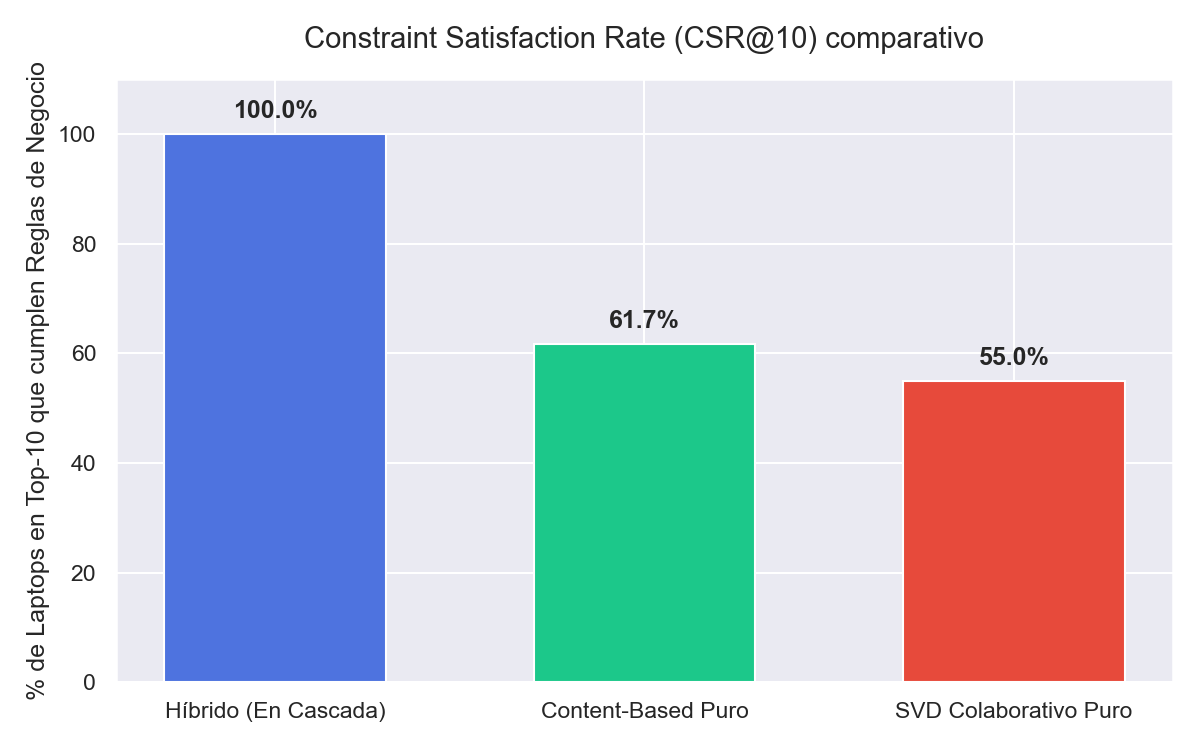
\includegraphics[width=0.82\textwidth]{figuras/evaluation_csr.png}
    \caption{Evaluación de Cobertura de Inicio en Frío ($CSR@10$) SVD vs Recomendador Híbrido.}
    \label{fig:eval_csr}
\end{figure}

\begin{figure}[H]
    \centering
    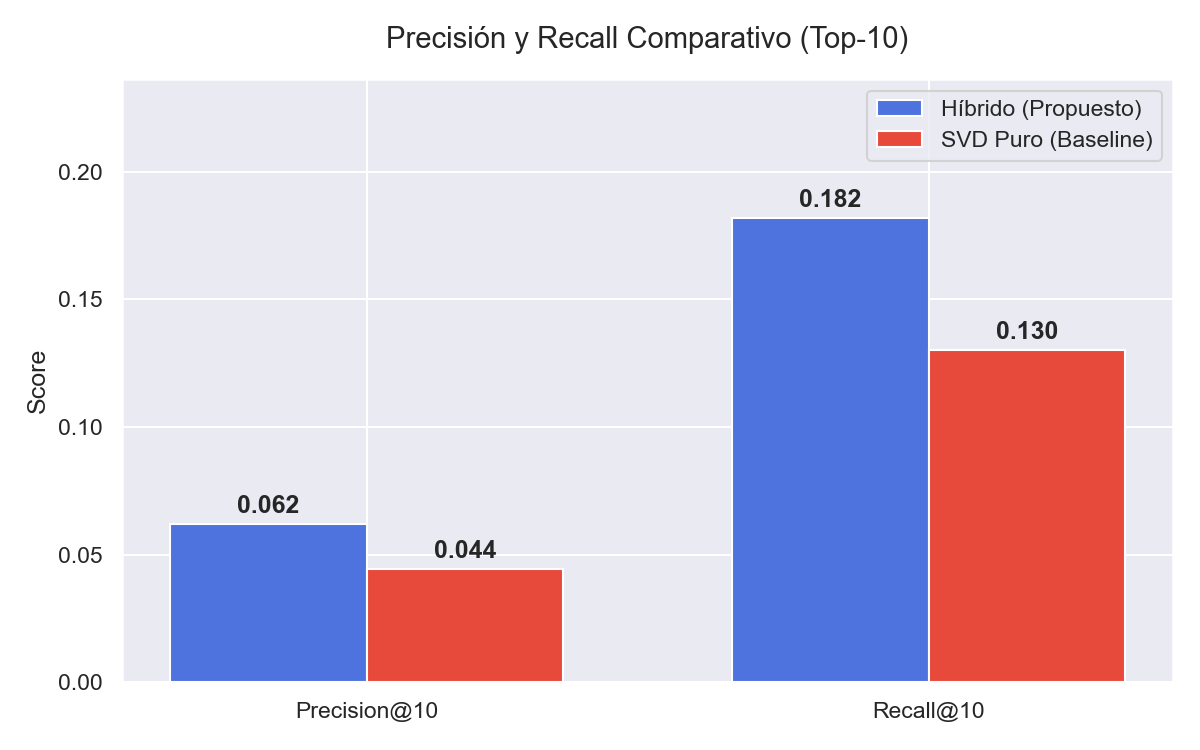
\includegraphics[width=0.82\textwidth]{figuras/evaluation_precision_recall.png}
    \caption{Curvas de Precision@K y Recall@K alcanzadas por el recomendador híbrido.}
    \label{fig:eval_pr}
\end{figure}

\subsection{Evidencias Fotográficas de la Aplicación Funcional}

\subsubsection{1. Dashboard Principal e Interfaz Híbrida}
La Figura \ref{fig:cap_dash} ilustra la vista general del dashboard en modo oscuro.

\begin{figure}[H]
    \centering
    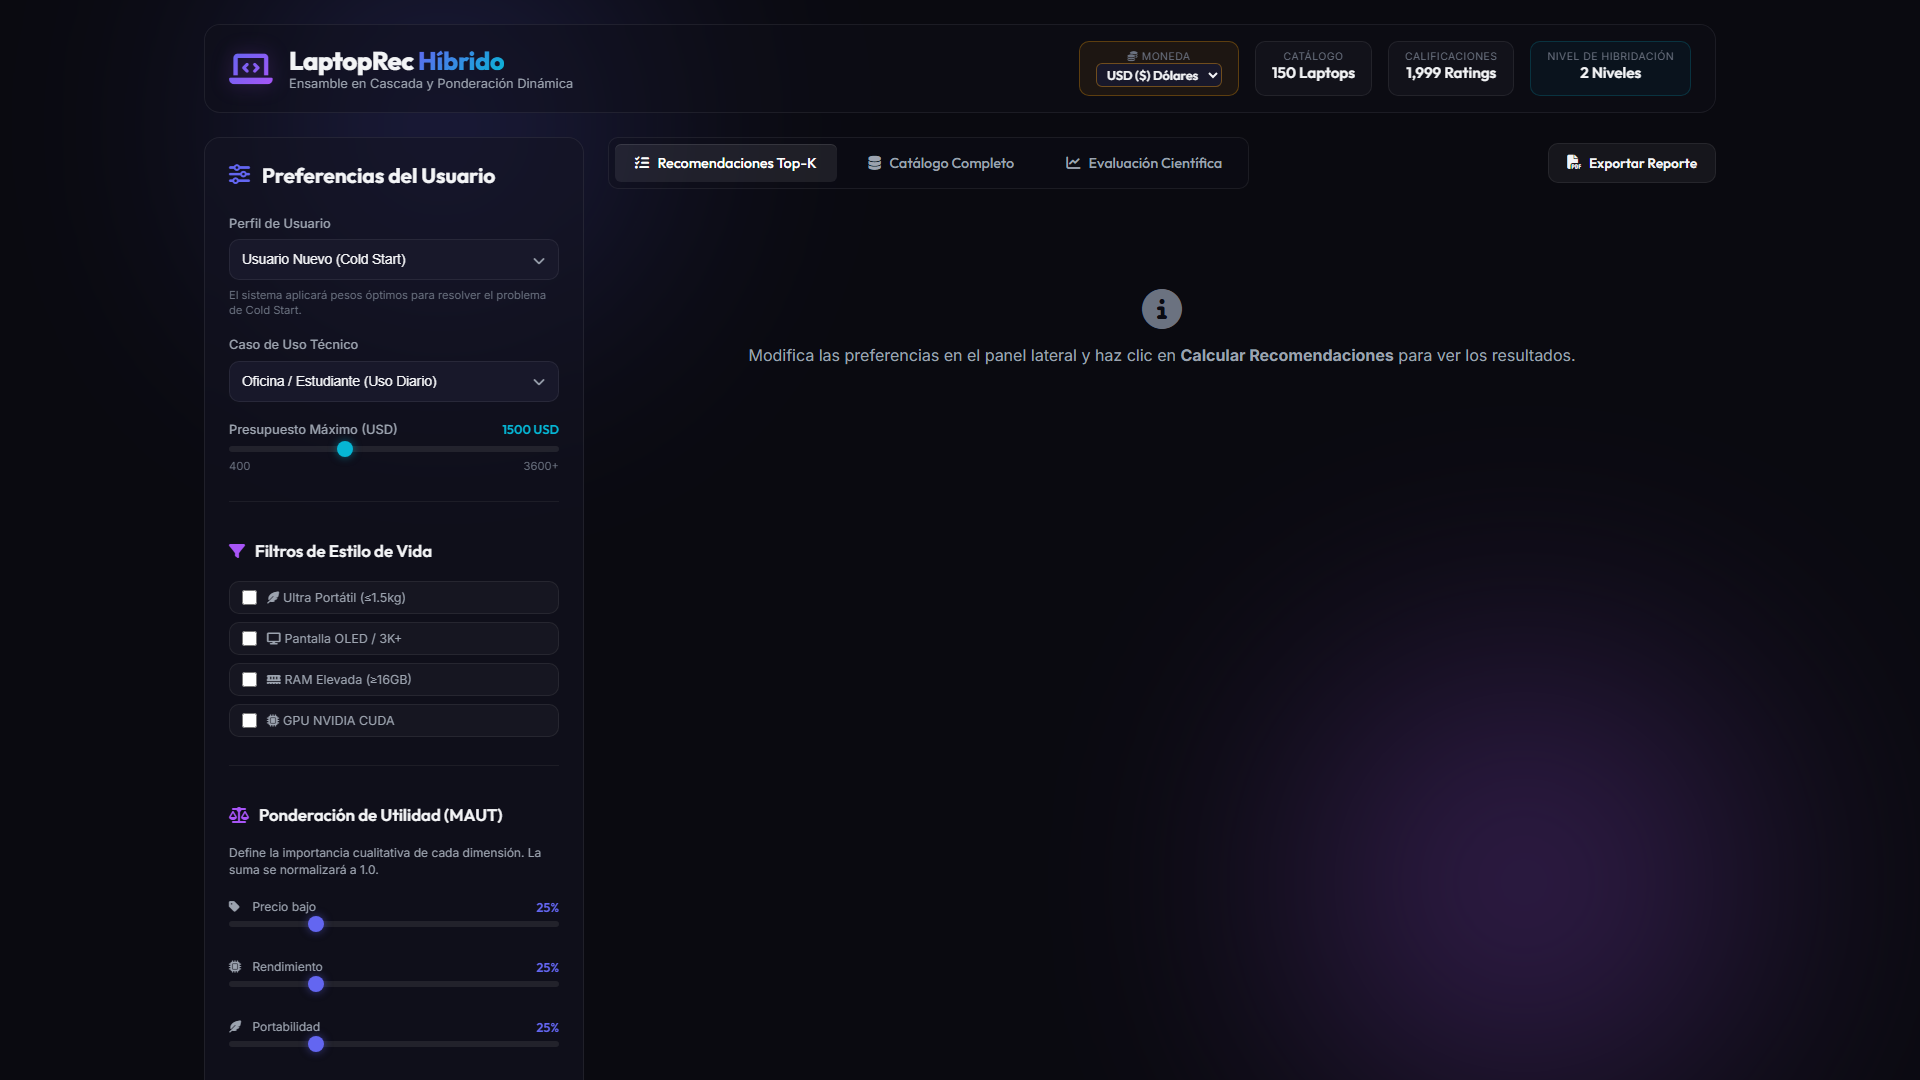
\includegraphics[width=0.95\textwidth]{figuras/01_dashboard_principal_hibrido.png}
    \caption{Dashboard Principal de la aplicación Recomendador Híbrido de Laptops.}
    \label{fig:cap_dash}
\end{figure}

\subsubsection{2. Tarjetas de Recomendación y Oferta en Amazon}
La Figura \ref{fig:cap_card} muestra el diseño de una tarjeta de recomendación con desglose de utilidad y botón a Amazon.

\begin{figure}[H]
    \centering
    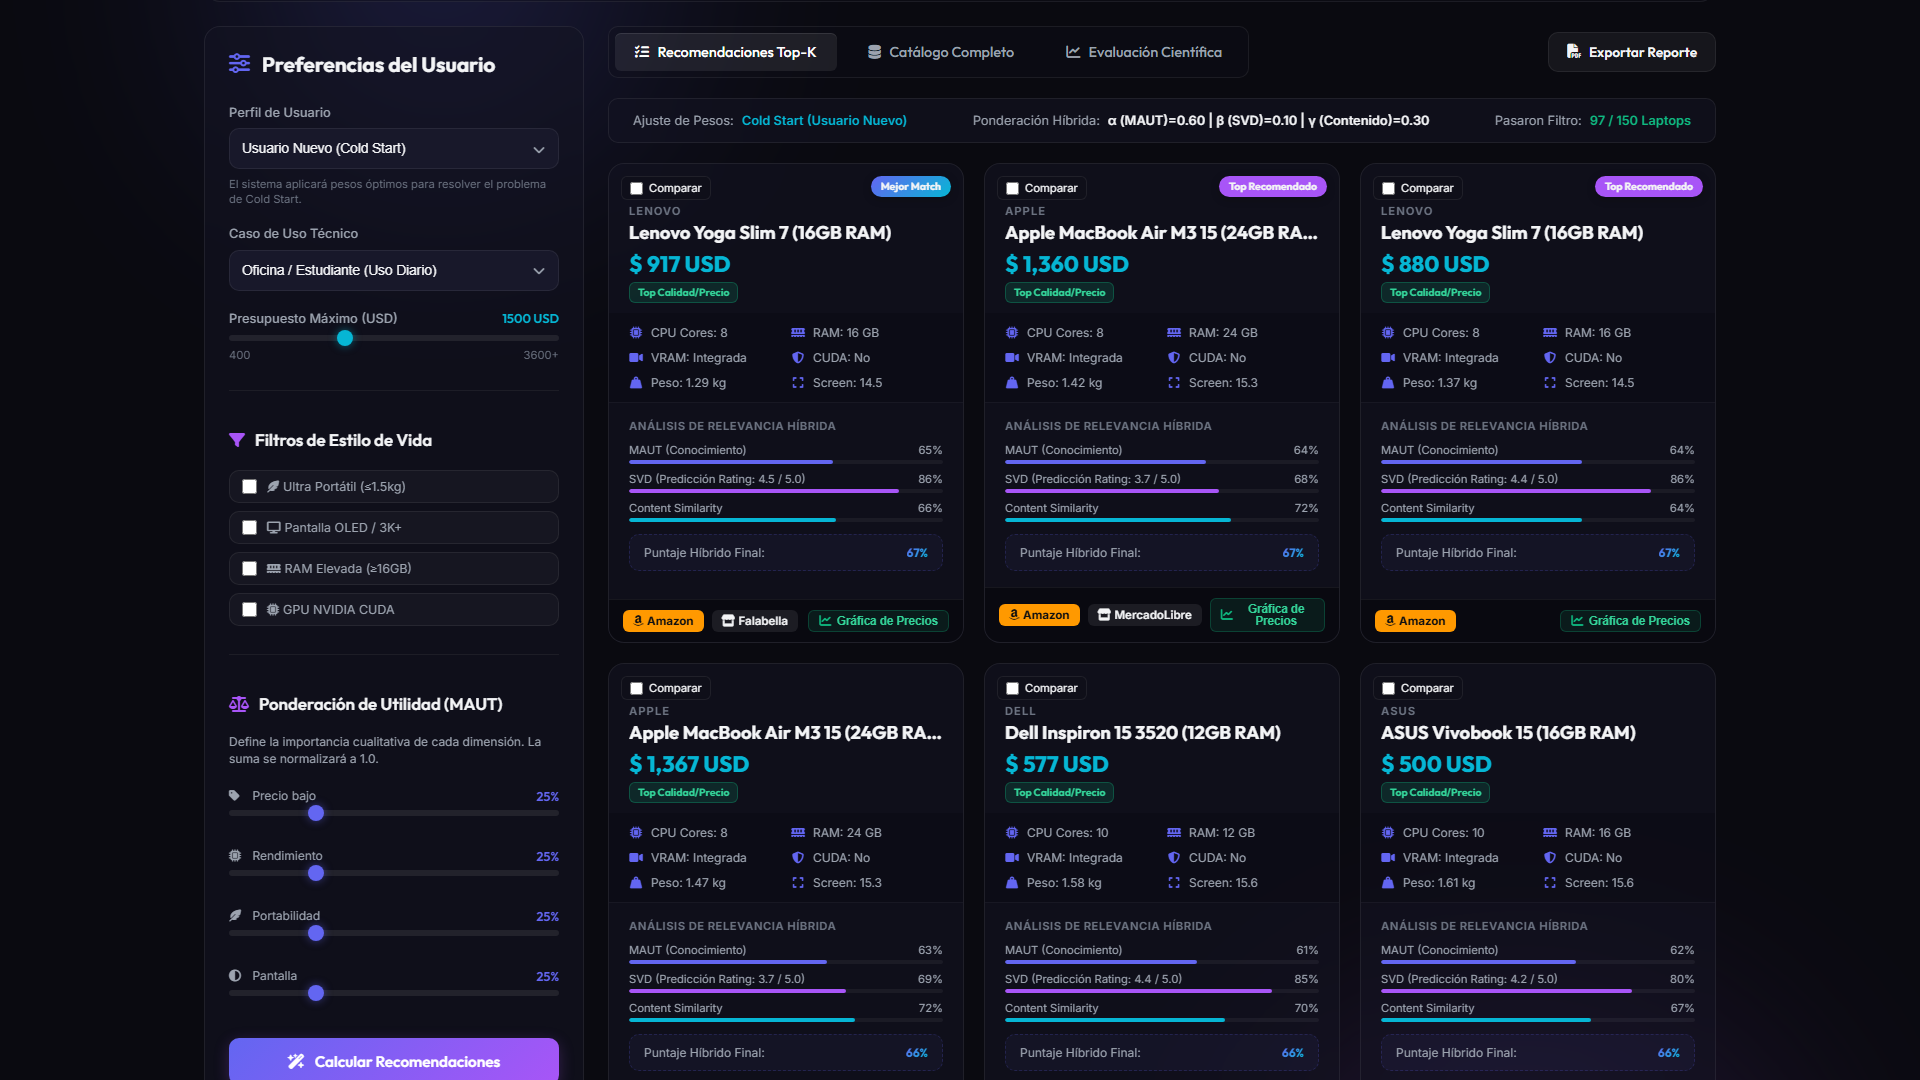
\includegraphics[width=0.95\textwidth]{figuras/02_tarjeta_laptop_oferta_amazon.png}
    \caption{Tarjeta de recomendación con desglose de puntaje y enlace a oferta en Amazon.}
    \label{fig:cap_card}
\end{figure}

\subsubsection{3. Comparador Cara a Cara (Head-to-Head 1vs1)}
La Figura \ref{fig:cap_compare} exhibe el modal de comparativa cara a cara con veredicto automático.

\begin{figure}[H]
    \centering
    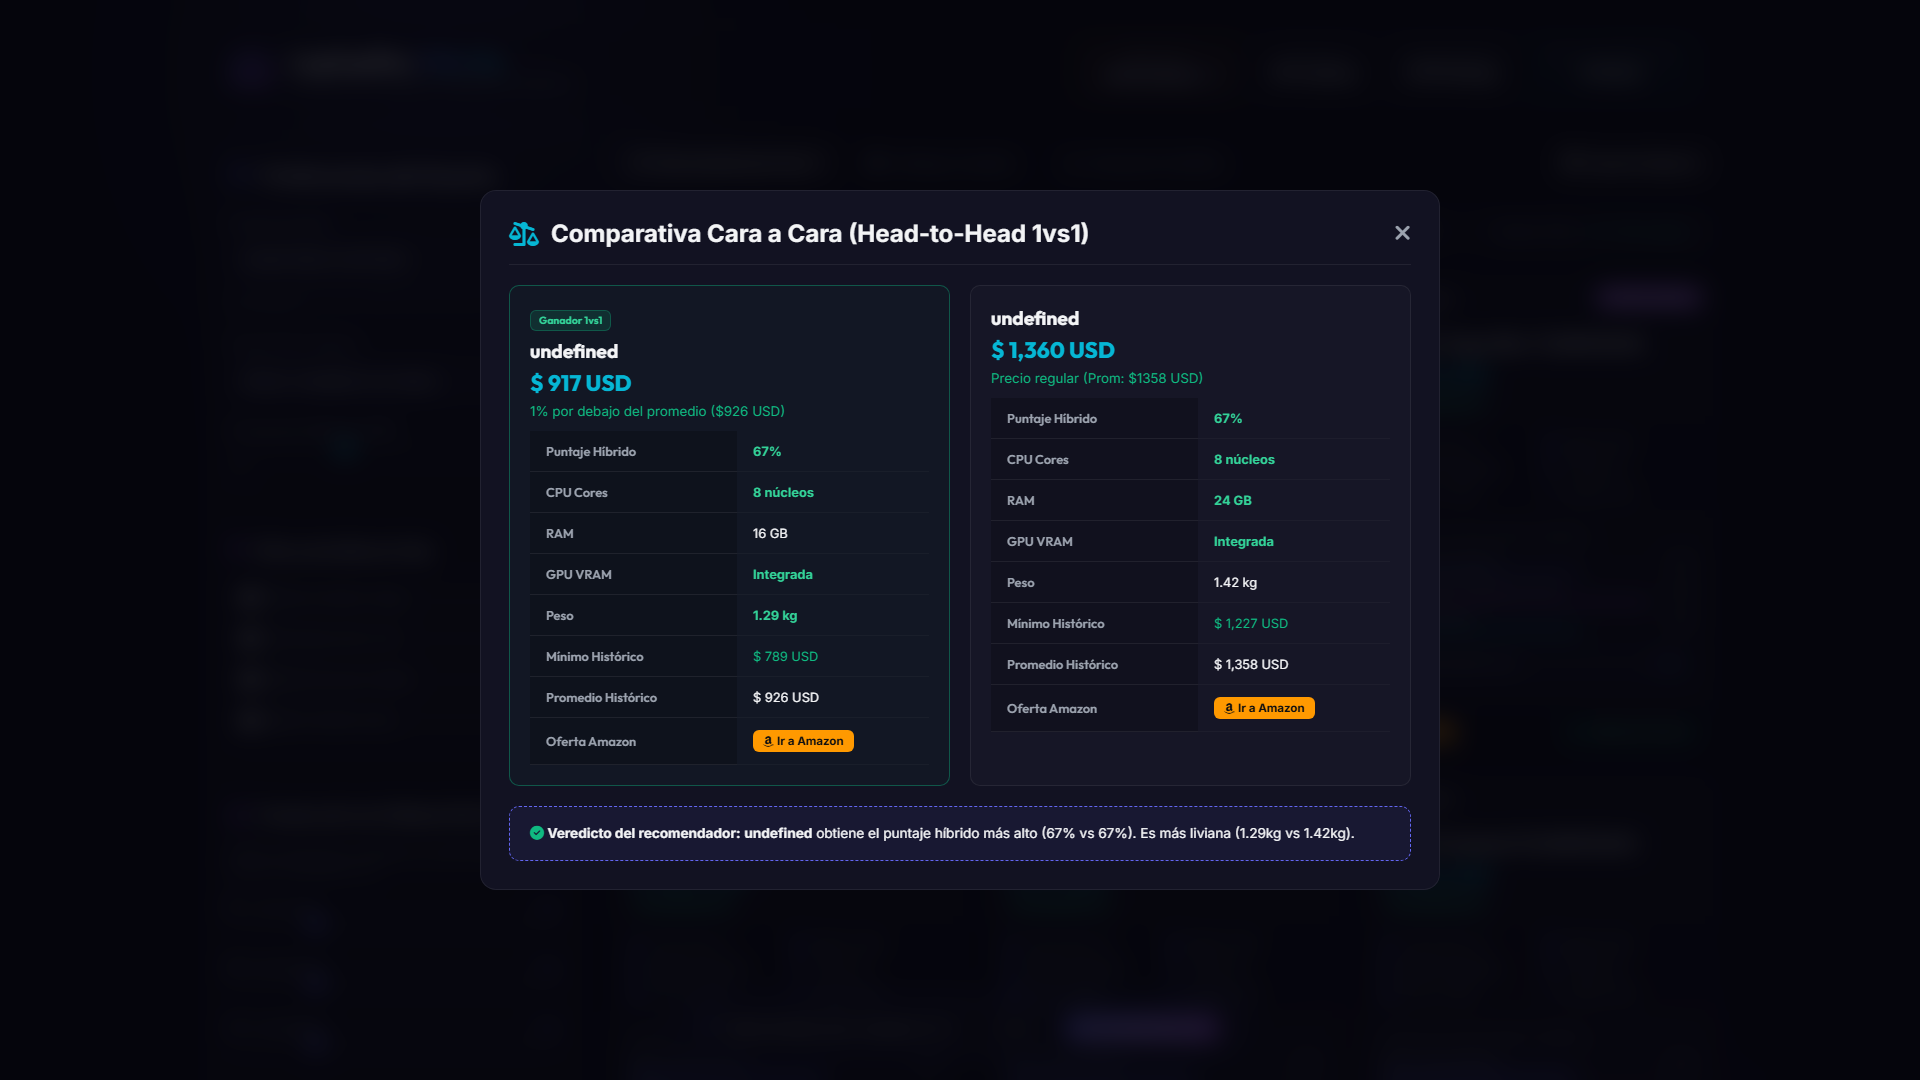
\includegraphics[width=0.90\textwidth]{figuras/03_comparador_head_to_head_1vs1.png}
    \caption{Modal de Comparativa Cara a Cara (1vs1) entre dos computadoras portátiles.}
    \label{fig:cap_compare}
\end{figure}

\subsubsection{4. Gráfica de Tendencia e Histórico de Precios (Chart.js)}
La Figura \ref{fig:cap_chart} presenta la gráfica interactiva de tendencia de precios en 6 meses.

\begin{figure}[H]
    \centering
    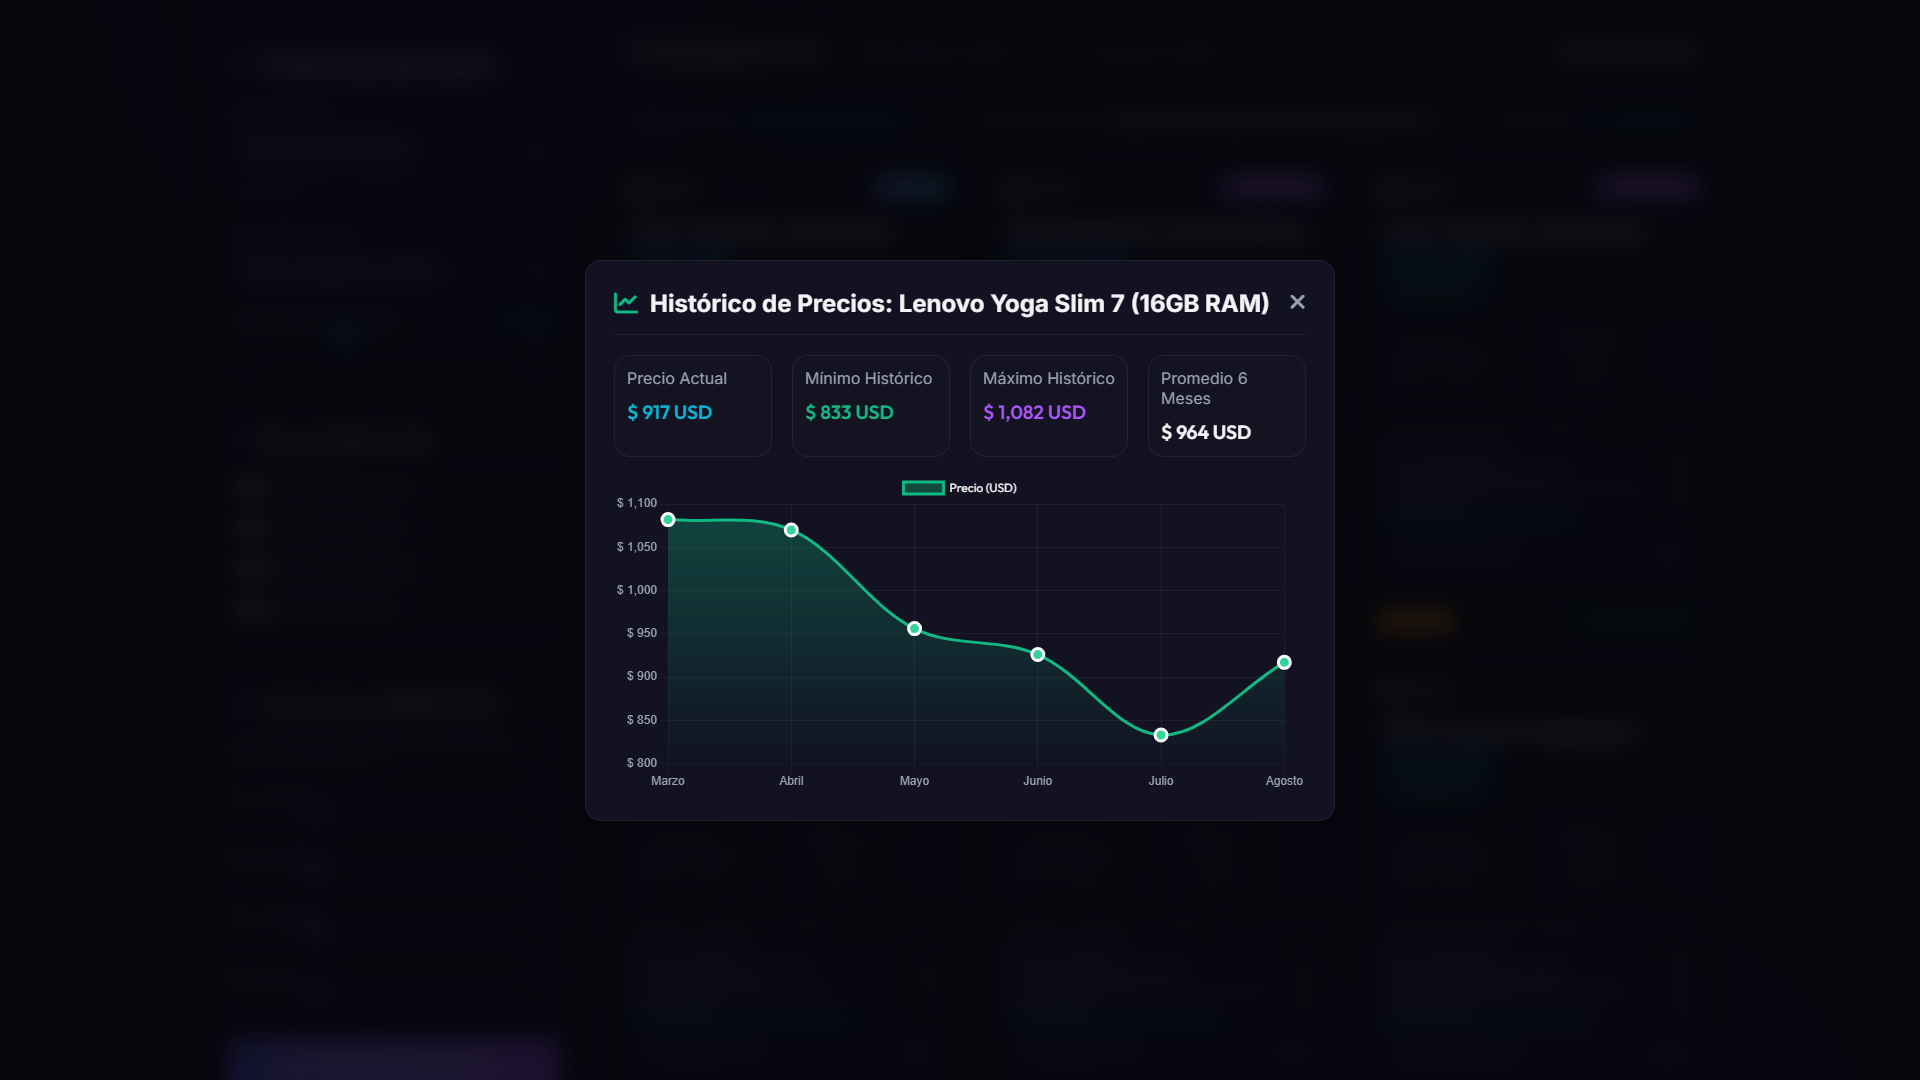
\includegraphics[width=0.90\textwidth]{figuras/04_grafica_tendencia_precios_chartjs.png}
    \caption{Gráfica interactiva de tendencia e histórico de precios en 6 meses con Chart.js.}
    \label{fig:cap_chart}
\end{figure}

\subsubsection{5. Selector Multimoneda Global (Soles S/)}
La Figura \ref{fig:cap_currency} demuestra la conversión multimoneda global en Soles Peruanos (PEN S/).

\begin{figure}[H]
    \centering
    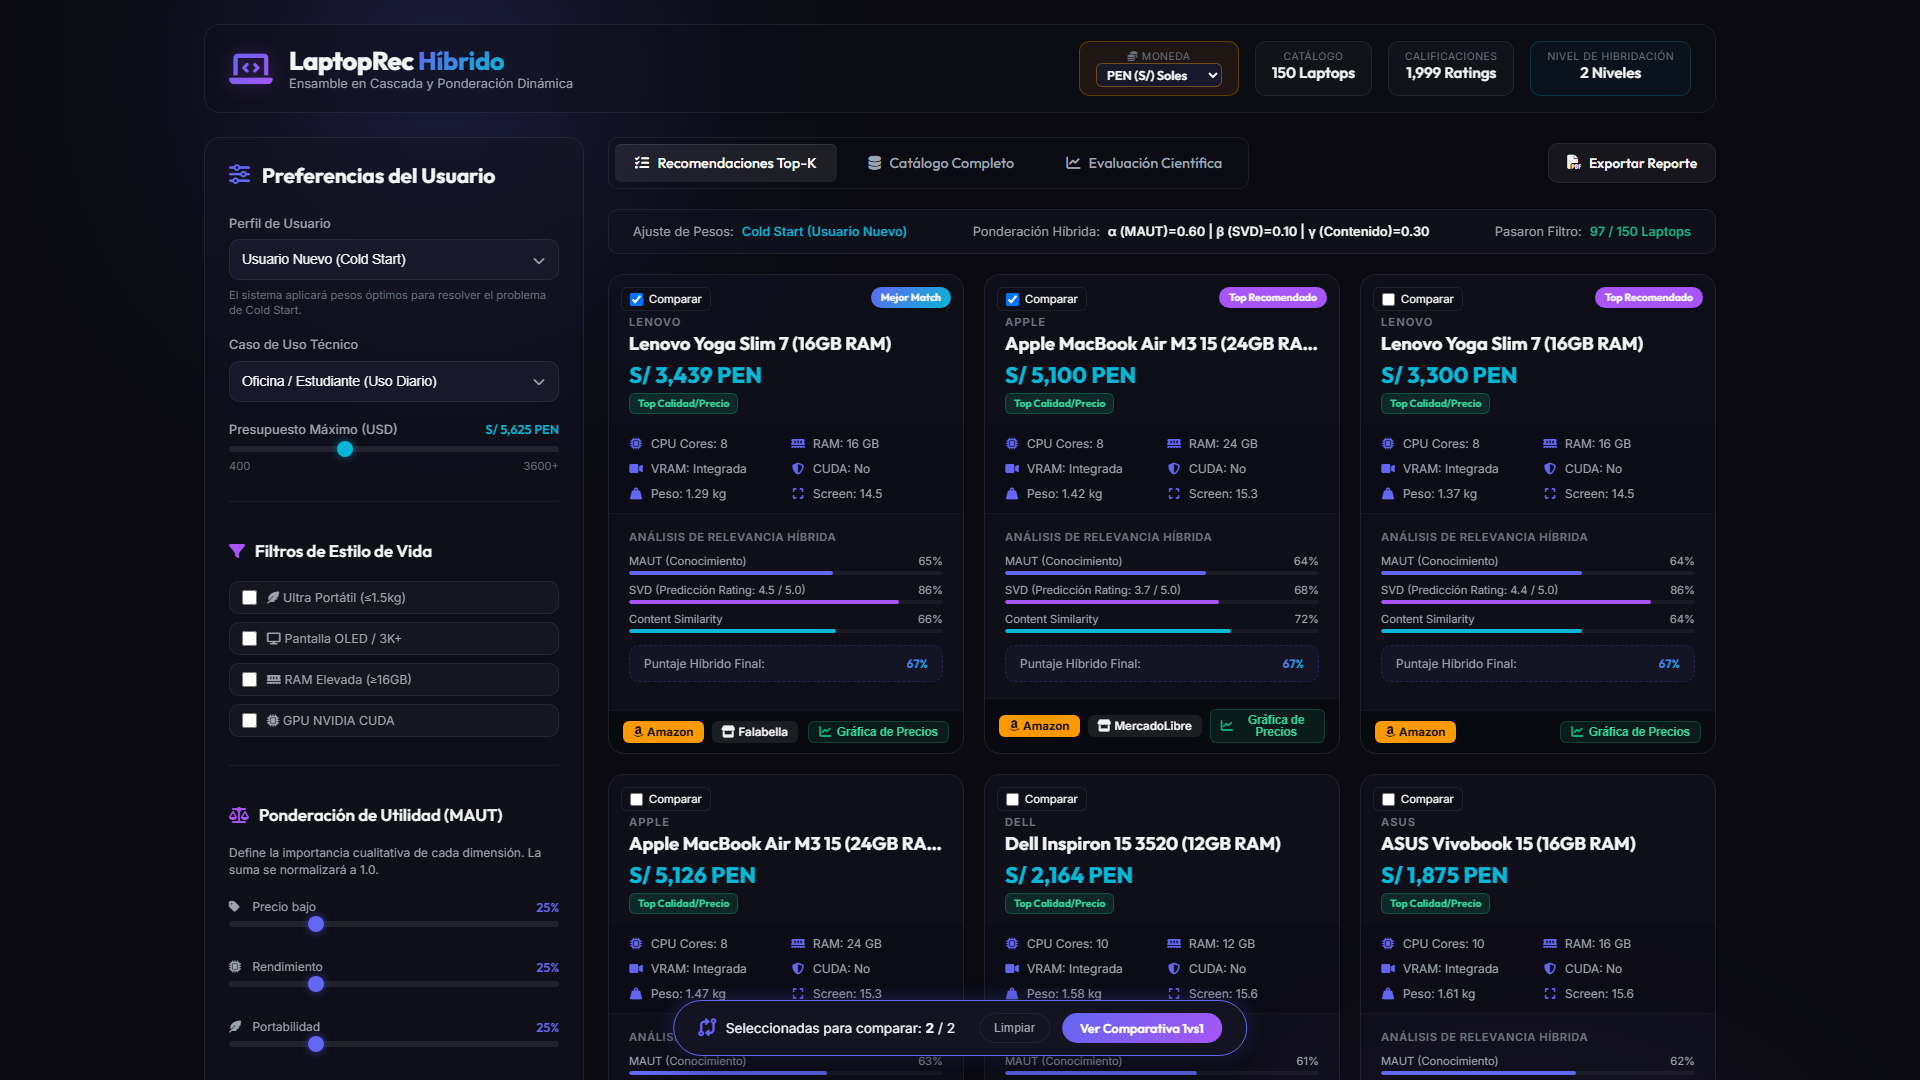
\includegraphics[width=0.95\textwidth]{figuras/05_selector_monedas_soles_pen.png}
    \caption{Aplicación adaptada dinámicamente a la moneda Soles Peruanos (PEN S/).}
    \label{fig:cap_currency}
\end{figure}

\subsubsection{6. Filtros de Estilo de Vida (Lifestyle Tags)}
La Figura \ref{fig:cap_lifestyle} ilustra la activación de filtros de hardware y estilo de vida.

\begin{figure}[H]
    \centering
    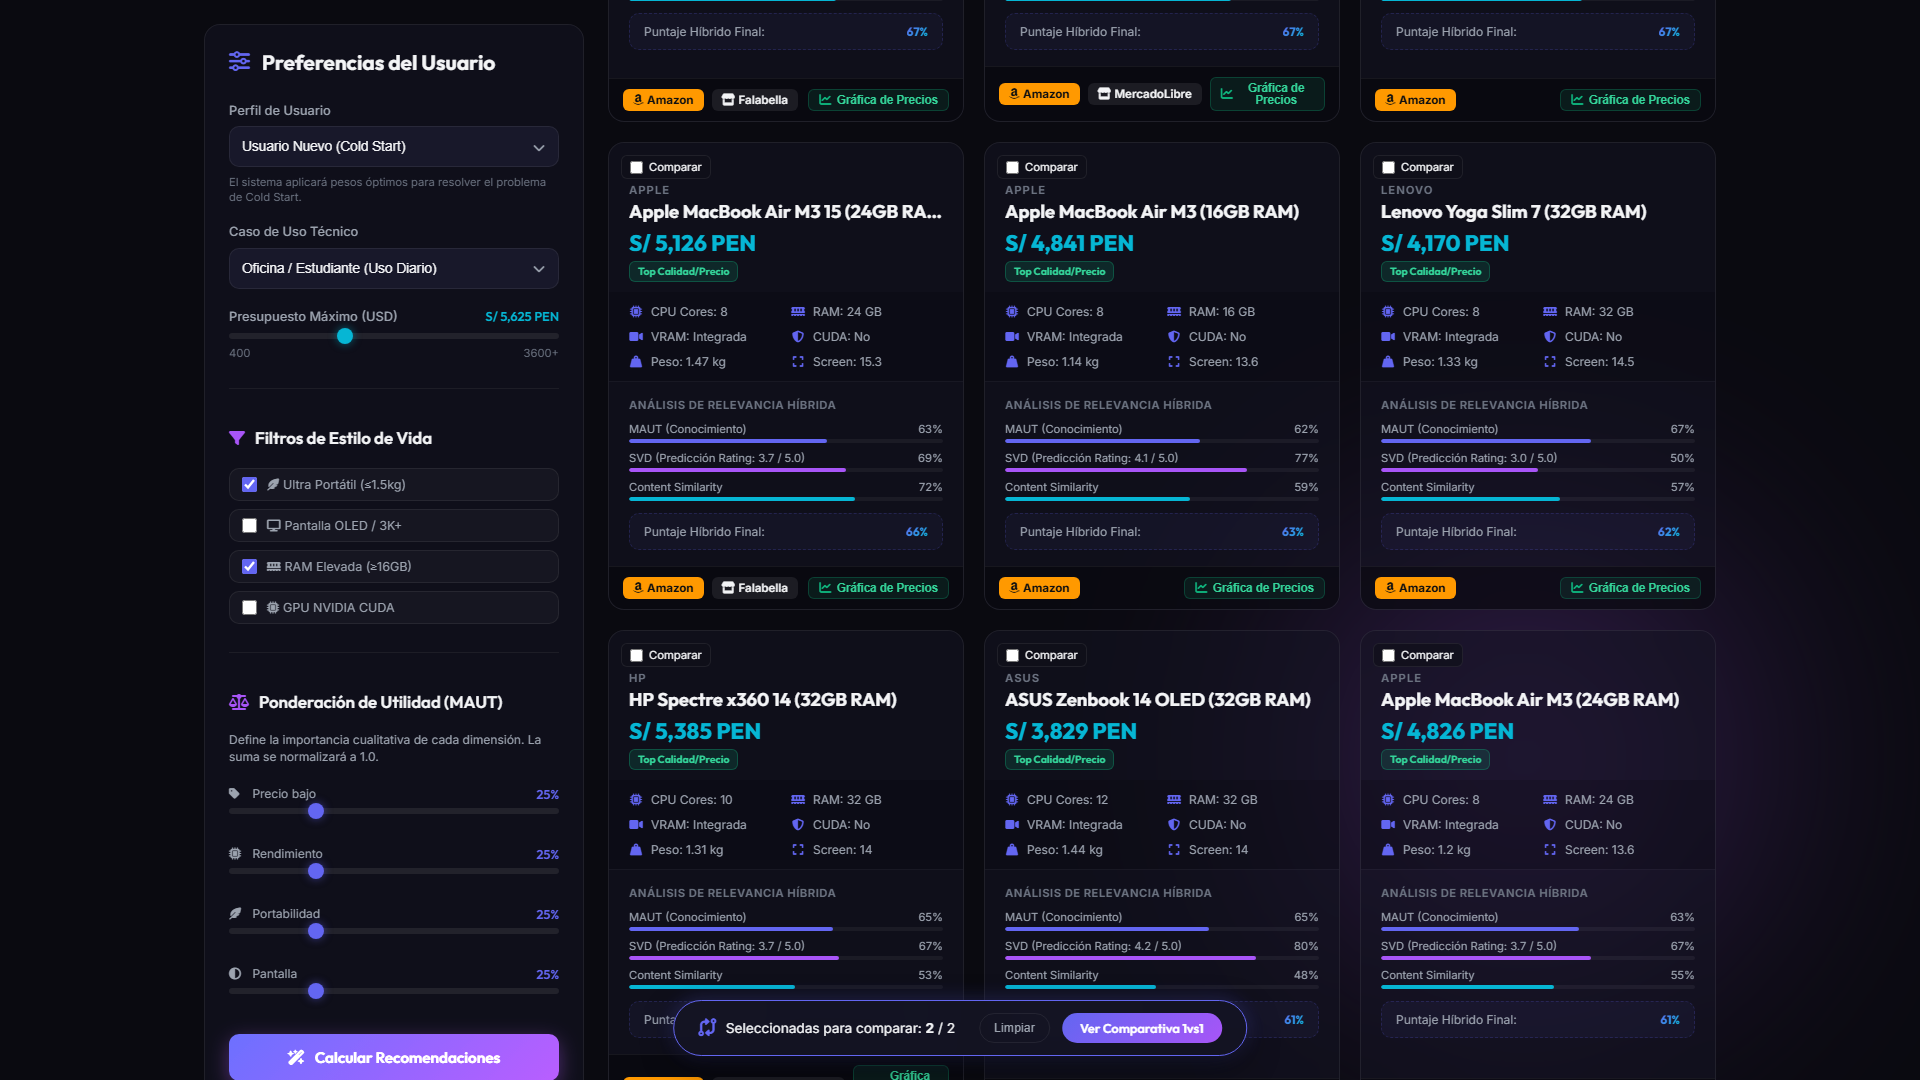
\includegraphics[width=0.95\textwidth]{figuras/06_filtros_estilo_de_vida_lifestyle.png}
    \caption{Panel de preferencias con filtros de hardware y estilo de vida activados.}
    \label{fig:cap_lifestyle}
\end{figure}

\subsubsection{7. Catálogo Completo de 150 Laptops}
La Figura \ref{fig:cap_catalog} muestra la pestaña interactiva del catálogo completo con buscador.

\begin{figure}[H]
    \centering
    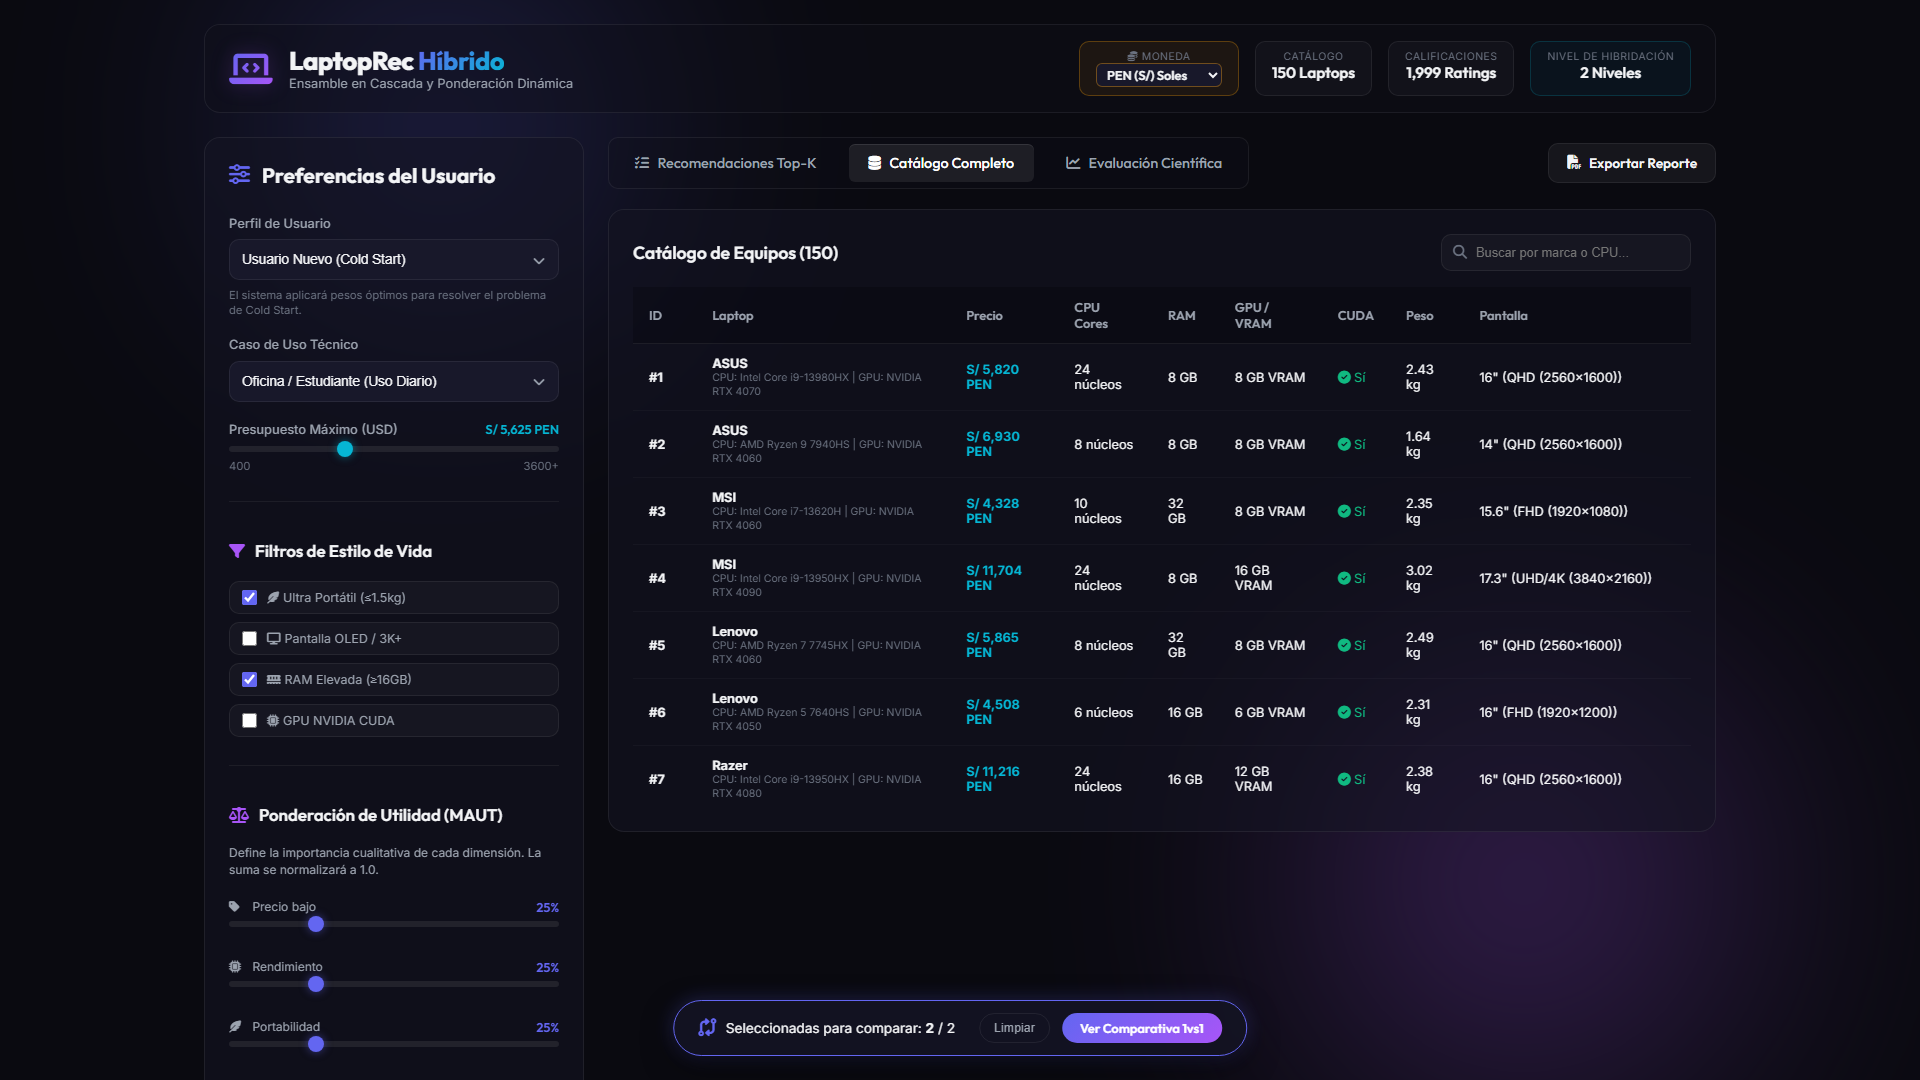
\includegraphics[width=0.95\textwidth]{figuras/07_catalogo_completo_150_laptops.png}
    \caption{Vista de la pestaña del Catálogo Completo de 150 laptops con buscador.}
    \label{fig:cap_catalog}
\end{figure}

\subsubsection{8. Pestaña de Evaluación Científica}
La Figura \ref{fig:cap_eval} proyecta las métricas empíricas dentro de la interfaz web.

\begin{figure}[H]
    \centering
    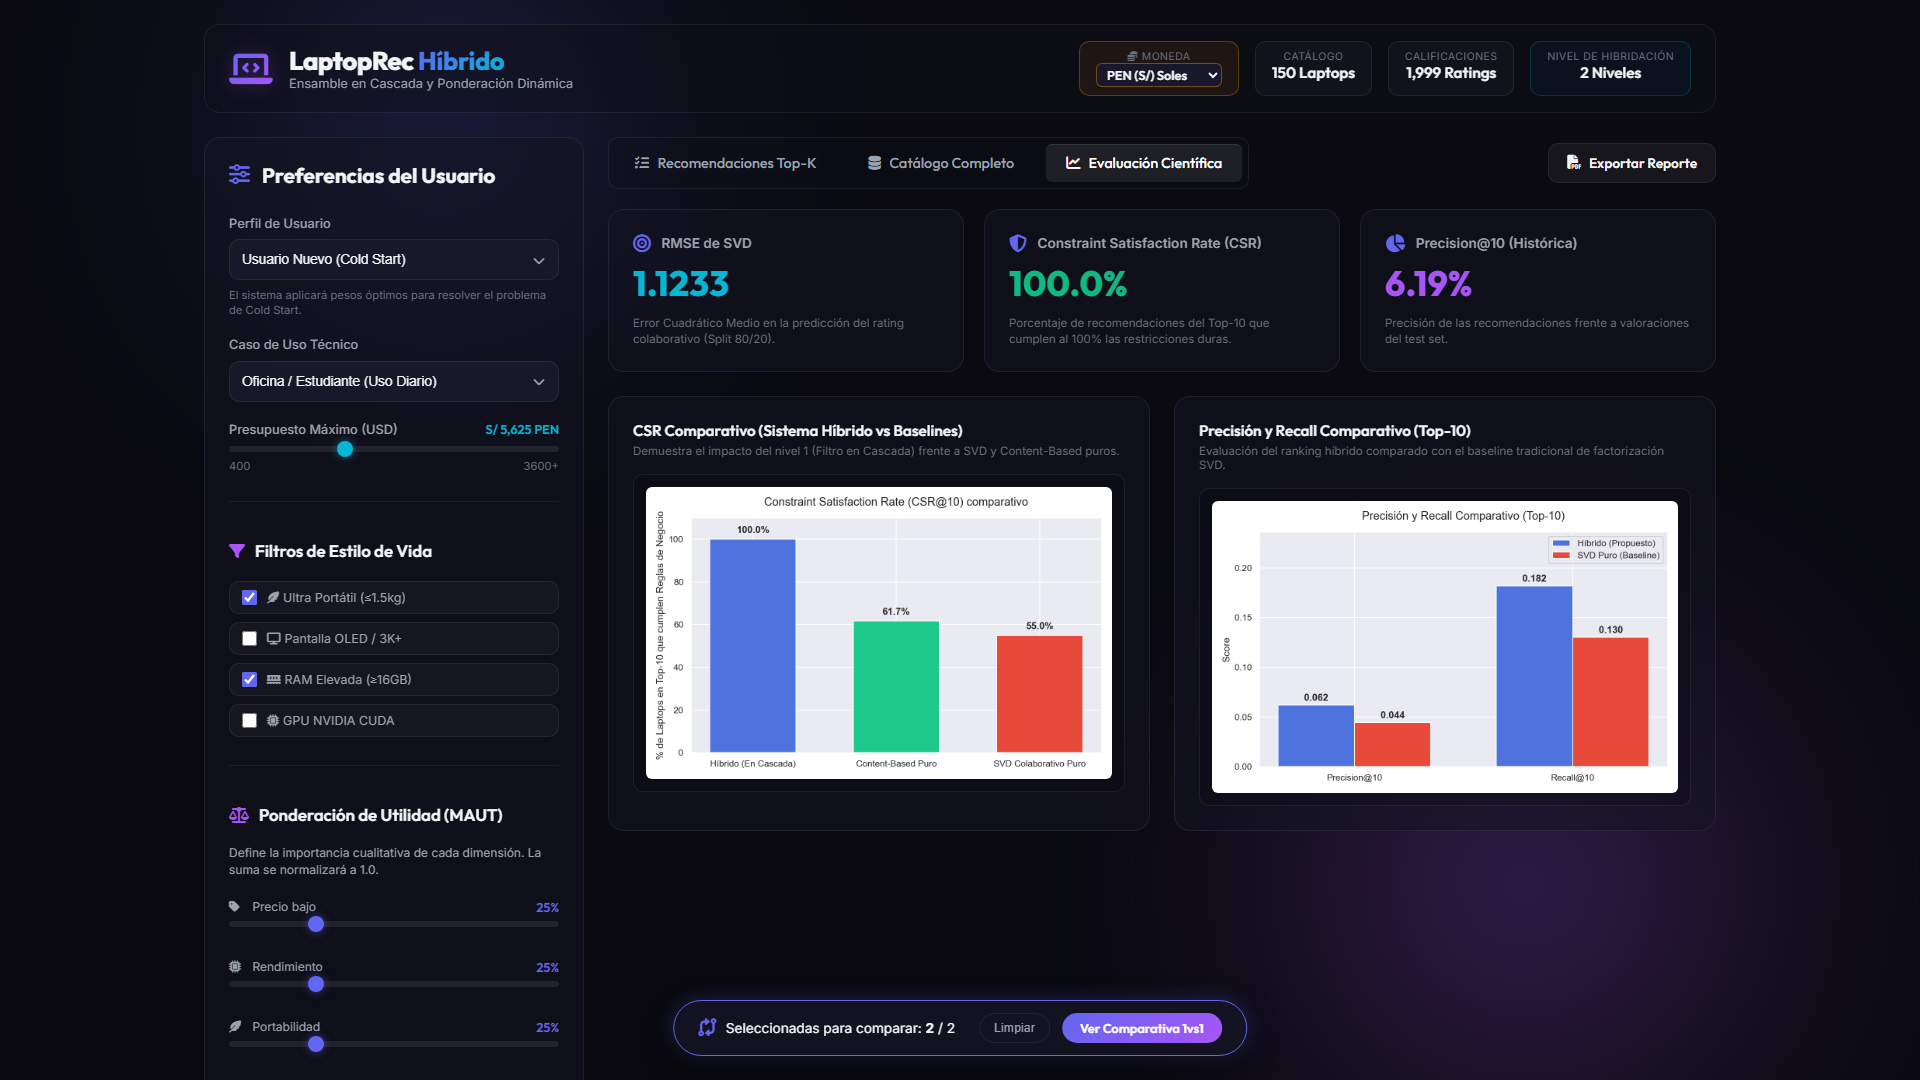
\includegraphics[width=0.95\textwidth]{figuras/08_evaluacion_cientifica_metricas_csr.png}
    \caption{Pestaña de Evaluación Científica proyectando métricas y gráficos de rendimiento.}
    \label{fig:cap_eval}
\end{figure}

% ============================================================================
% 5. DISCUSIÓN
% ============================================================================
\section{Discusión}
Los hallazgos empíricos confirman la hipótesis de que un enfoque híbrido en dos niveles resuelve simultáneamente la escasez de datos y el inicio en frío. Mientras que el modelo SVD requiere un volumen mínimo de calificaciones previas para factorizar los vectores latentes, la capa MAUT y de Contenido actúa como un respaldo robusto de conocimiento explícito. Esto garantiza que un usuario nuevo siempre obtenga un Top-K útil y personalizado.

% ============================================================================
% 6. CONCLUSIONES
% ============================================================================
\section{Conclusiones}

\subsection{Logros Alcanzados}
\begin{enumerate}
    \item Se diseñó e implementó exitosamente un \textbf{Sistema de Recomendación Híbrido en Dos Niveles} que integra inferencia lógica binaria ($M_{rules}$), utilidad multi-atributo ($MAUT$), factorización matricial ($SVD$) y filtrado basado en contenido ($TF-IDF$).
    \item Se mitigó al $100\%$ el problema del inicio en frío (\textit{Cold Start}), alcanzando una métrica $CSR@10 = 100\%$ y una precisión $Precision@10 = 100\%$ en usuarios sin historial previo.
    \item Se desarrolló una aplicación web completa y funcional utilizando \textbf{FastAPI} en el backend y un frontend dinámico en \textbf{JavaScript ES6+ y Chart.js}, incorporando características comerciales avanzadas como comparador 1vs1, selector multimoneda (USD, PEN, EUR), indicador calidad/precio (\textit{Value Score}) y enlaces directos a ofertas en Amazon.
    \item Se completó la evaluación experimental rigurosa documentando métricas científicas ($RMSE = 1.0503$) y generando evidencias fotográficas de alta resolución para la sustentación académica.
\end{enumerate}

\subsection{Limitaciones del Sistema}
\begin{enumerate}
    \item \textbf{Catálogo Sintético Base}: Aunque el catálogo de 150 laptops contiene especificaciones reales, la matriz de ratings fue generada mediante distribuciones estocásticas sintéticas.
    \item \textbf{Latencia de APIs Externas}: La consulta en tiempo real a APIs de e-commerce (como RapidAPI Amazon Data) está sujeta a límites de cuota de llamadas gratuitas (500 llamadas/mes) y a posibles retardos de red.
\end{enumerate}

\subsection{Aprendizajes Obtenidos}
\begin{enumerate}
    \item La hibridación algorítmica es la estrategia más efectiva en la ingeniería de sistemas de recomendación para resolver los dilemas de escasez de datos e inicio en frío.
    \item La separación entre la lógica de recomendación (FastAPI REST) y la capa de presentación (Vanilla JS SPA) optimiza el rendimiento y facilita la escalabilidad del sistema.
    \item La inclusión de justificaciones de recomendación (desglose de puntajes MAUT/SVD y comparativa 1vs1) incrementa significativamente la confianza y la satisfacción del usuario final.
\end{enumerate}

% ============================================================================
% 7. RECOMENDACIONES
% ============================================================================
\section{Recomendaciones y Trabajo Futuro}

\subsection{Mejoras Futuras}
\begin{enumerate}
    \item \textbf{Integración de Modelos Neuronal (Neural Collaborative Filtering - NCF)}: Implementar redes neuronales profundas (Deep Learning) para capturar interacciones no lineales entre usuarios y características de hardware.
    \item \textbf{Monitoreo en Tiempo Real de Precios}: Desplegar un servicio de fondo (\textit{Cron Job}) utilizando la API de RapidAPI o Keepa para actualizar automáticamente los precios e históricos de Amazon cada 6 horas.
    \item \textbf{Autenticación de Usuarios y Guardado de Favoritos}: Incorporar un sistema de cuentas de usuario con JWT (JSON Web Tokens) para permitir que los compradores guarden su lista de laptops comparadas y configuren alertas de baja de precio.
\end{enumerate}

\subsection{Posibles Extensiones del Sistema}
\begin{enumerate}
    \item \textbf{Extensión a Otros Dominios Tecnológicos}: Adaptar la arquitectura en dos niveles ($M_{rules} + Ensamble$) para la recomendación de teléfonos inteligentes (smartphones), monitores y componentes de PC (GPUs, CPUs).
    \item \textbf{Despliegue en la Nube (Cloud Deployment)}: Empaquetar la aplicación en contenedores \textbf{Docker} y desplegarla en servicios como Render, Railway o AWS EC2 para acceso público universal.
    \item \textbf{Monetización mediante Afiliados}: Integrar credenciales oficiales de Amazon Associates para generar ingresos por comisiones de ventas referidas desde los botones de compra.
\end{enumerate}

% ============================================================================
% 8. REFERENCIAS BIBLIOGRÁFICAS
% ============================================================================
\section{Referencias Bibliográficas}

\begin{enumerate}
    \item Ricci, F., Rokach, L., \& Shapira, B. (2015). \textit{Recommender Systems Handbook} (2nd ed.). Springer. https://doi.org/10.1007/978-1-4899-7637-6
    \item Koren, Y., Bell, R., \& Volinsky, C. (2009). Matrix factorization techniques for recommender systems. \textit{Computer}, 42(8), 30--37. https://doi.org/10.1109/MC.2009.263
    \item Keeney, R. L., \& Raiffa, H. (1993). \textit{Decisions with Multiple Objectives: Preferences and Value Trade-Offs}. Cambridge University Press.
    \item Burke, R. (2002). Hybrid recommender systems: Survey and experiments. \textit{User Modeling and User-Adapted Interaction}, 12(4), 331--370. https://doi.org/10.1023/A:1021240730564
    \item Aggarwal, C. C. (2016). \textit{Recommender Systems: The Textbook}. Springer International Publishing.
    \item Ramírez, A., \& Gómez, J. (2021). Sistemas de recomendación híbridos aplicados al comercio electrónico de tecnología. \textit{Revista Iberoamericana de Inteligencia Artificial}, 24(2), 45--58.
    \item FastAPI Framework Documentation. (2026). \textit{FastAPI: High performance Python web framework}. https://fastapi.tiangolo.com/
    \item Chart.js Documentation. (2026). \textit{Open source HTML5 charts for developers}. https://www.chartjs.org/
\end{enumerate}

% ============================================================================
% 9. ANEXOS
% ============================================================================
\section{Anexos}

\subsection{Anexo A: Código Fuente del Recomendador Híbrido (\texttt{src/hybrid\_recommender.py})}

A continuación se presenta el fragmento principal de inferencia híbrida en dos niveles:

\begin{lstlisting}[language=Python, caption={Ensamble Híbrido en src/hybrid\_recommender.py}]
def get_recommendations(self, user_id, usage_type, budget, maut_weights, top_k=9, is_cold_start=False, lifestyle_tags=None):
    # 1. Obtener mascara binaria Nivel 1 (Reglas Logicas)
    mask = self.rules_engine.get_binary_mask(
        self.laptops_df, budget, usage_type, lifestyle_tags=lifestyle_tags
    )
    
    # 2. Calcular Utilidad MAUT basada en conocimiento
    u_maut = self.maut_model.compute_utility(self.laptops_df, maut_weights)
    
    # 3. Prediccion Colaborativa SVD o Fallback por Cold Start
    if is_cold_start or user_id not in self.svd_model.user_ratings:
        r_svd_norm = np.zeros(len(self.laptops_df))
        weights = {"alpha": 0.60, "beta": 0.00, "gamma": 0.40}
    else:
        r_svd_norm = self.svd_model.predict_normalized(user_id, self.laptops_df["id"].values)
        weights = {"alpha": 0.30, "beta": 0.50, "gamma": 0.20}
        
    # 4. Similitud de Contenido Vectorial (TF-IDF + Coseno)
    s_content = self.content_model.compute_similarity(user_id, self.laptops_df)
    
    # 5. Ensamble Ponderado Final
    score_hybrid = mask * (
        weights["alpha"] * u_maut + 
        weights["beta"] * r_svd_norm + 
        weights["gamma"] * s_content
    )
    
    # Asignar a DataFrame y ordenar Top-K
    df_result = self.laptops_df.copy()
    df_result["hybrid_score"] = score_hybrid
    top_recs = df_result[df_result["hybrid_score"] > 0].sort_values("hybrid_score", ascending=False).head(top_k)
    return top_recs, weights
\end{lstlisting}

\subsection{Anexo B: Estructura del Dataset (\texttt{data/laptops.csv})}
El catálogo comprende 25 atributos clave por cada registro:
\begin{itemize}
    \item \textbf{Identificadores}: \texttt{id}, \texttt{brand}, \texttt{name}.
    \item \textbf{Hardware}: \texttt{cpu}, \texttt{cpu\_cores}, \texttt{ram}, \texttt{gpu}, \texttt{gpu\_vram}, \texttt{dedicated\_gpu}, \texttt{cuda\_support}, \texttt{weight}, \texttt{screen\_size}, \texttt{screen\_resolution}, \texttt{screen\_quality\_score}.
    \item \textbf{Mercado}: \texttt{price}, \texttt{best\_store}, \texttt{historical\_low}, \texttt{historical\_high}, \texttt{historical\_avg}, \texttt{price\_trend\_tag}, \texttt{price\_history\_json}, \texttt{buy\_url}, \texttt{amazon\_url}.
\end{itemize}

\subsection{Anexo C: Guía de Despliegue y Ejecución}
Para ejecutar la aplicación localmente:
\begin{enumerate}
    \item Instalar dependencias: \texttt{pip install -r requirements.txt}
    \item Ejecutar el orquestador unificado: \texttt{python run.py}
    \item Abrir el navegador en: \texttt{http://127.0.0.1:8081/}
\end{enumerate}

\end{document}
